\documentclass[conference]{IEEEtran}
\IEEEoverridecommandlockouts

\newcommand{\prof}[1]{{\leavevmode\color{red}[#1]}}
%\newcommand{\prof}[1]{\textbf{\color{red} [#1]}}
\newcommand{\my}[1]{{\leavevmode\color{blue}#1}}

\newcommand{\Fact}{Fact}
\newcommand{\fact}{fact}
\newcommand{\Explanation}{Explanation}
\newcommand{\explanation}{explanation}

\newcommand{\evaluator}{Index Evaluator}
\newcommand{\solution}{hierarchical Intervention}

\newcommand{\intensity}{intensity}
\newcommand{\influence}{influence}
\newcommand{\newvalue}{\textit{explanation index}}

%%% To be removed or tested %%%
\newcommand{\aggravation}{Aggravation}
\newcommand{\intervention}{Intervention}

\usepackage{cite}
\usepackage{amsmath,amssymb,amsfonts}
\usepackage{graphicx}
\usepackage{textcomp}
\usepackage{xcolor}
\usepackage{url}
\usepackage{subcaption}
\usepackage{hyperref}
\usepackage{tikz}
\usepackage{pgfplots}
\def\BibTeX{{\rm B\kern-.05em{\sc i\kern-.025em b}\kern-.08em
    T\kern-.1667em\lower.7ex\hbox{E}\kern-.125emX}}


\usepackage{booktabs} % For formal tables
\usepackage{color}

\usepackage{algorithm}
\usepackage{algpseudocode}
\usepackage{listings}
\usepackage{color}
\usepackage[labelsep=colon]{caption}
\usepackage{mathrsfs}

\usepackage{amsmath}
\definecolor{codegreen}{rgb}{0,0.6,0}
\definecolor{codegray}{rgb}{0.5,0.5,0.5}
\definecolor{codepurple}{rgb}{0.58,0,0.82}
\definecolor{backcolour}{rgb}{0.95,0.95,0.92}



\title{An Automated Framework for Explaining Facts Extracted From Mobility Datasets}

\author{
\IEEEauthorblockN{Anique Tahir}
\IEEEauthorblockA{
%\textit{School of Computing, Informatics, and Decision Systems Engineering} \\
\textit{Arizona State University}\\
Tempe, USA \\
artahir@asu.edu}
\and
\IEEEauthorblockN{Mohamed Sarwat}
\IEEEauthorblockA{
%\textit{School of Computing, Informatics, and Decision Systems Engineering} \\
\textit{Arizona State University}\\
Tempe, USA \\
msarwat@asu.edu}
}


\begin{document}


\maketitle


\begin{abstract}
%In the last few years, there has been a tremendous increase in the use of big data. Most of this data is hard to understand because of its size and dimensions. The importance of this problem can be emphasized by the fact that Big Data Research and Development Initiative was announced by the United States administration in 2012 to address problems faced by the government. Various states and cities in the US gather spatial data about incidents like police calls for service.

When a data scientist analyzes mobility data (e.g., using a data visualization tool), she may find out some interesting facts in the dataset. An example of a {\fact} can be: ``The number of Taxi trips in NYC on January 23, 2016, dropped drastically as compared to other days of the same month". However, the data scientist may be left clueless if they cannot find a crisp {\explanation} to such a {\fact}. Furthermore, the tedious task of finding a {\explanation} by manually scraping the data becomes even impossible with big data. 
%In this paper, we present an automated framework which guides the data scientist to find spatial {\explanation}s for {\fact}s discovered on spatial data. The proposed framework formally represents a {\fact} as an arithmetic relationship between queries posted on the data. 
%The proposed framework introduces a taxonomy of Observation/Explanation 
Existing techniques are designed for non-spatial data which cannot be applied to spatial data because it does not consider the spatial proximity. In this paper, we propose an automatic framework which guides the data scientist to explain the {\fact} discovered from mobility data. Our approach expands on the aggravation and intervention techniques while using spatial partitioning/clustering to improve {\explanation}s for spatial data. Experiments show that the proposed approach outperforms the state-of-the-art approaches in finding the {\explanation} for {\fact}s extracted from NYC taxi real mobility dataset.
% in precision and recall while outperforming intervention in precision when finding explanations for observations made on a real NYC taxi dataset as well as a disease outbreak datasets.
%, there are a lot of differences. How can we explain what factors account for these differences? 
%If we define the observation as an arithmetic relationship between queries, 
%this kind of problem can be solved by aggravation or intervention. Aggravation views the value of our observation for different set of tuples while intervention looks at the value of the observation after removing sets of tuples. We call the predicates which represent these tuples, explanations. Observations by themselves have limited importance. For example, if we observe a large number of taxi trips in a specific area, we might ask the question: Why are there so many trips here? Explanations attempt to answer these kinds of questions.

%While aggravation and intervention are designed for non spatial data, we propose a new approach for explaining spatially heterogeneous data. Our approach expands on aggravation and intervention while using spatial partitioning/clustering to improve explanations for spatial data. Our proposed approach was evaluated against a real-world taxi dataset as well as a synthetic disease outbreak datasets. The approach was found to outperform aggravation in precision and recall while outperforming intervention in precision.
\end{abstract}



\label{sec:Intro}
\section{Introduction}

%When we analyze data, we might make some observations that pique our curiousity and then try to find out a reason for specific observations. 
When a data scientist analyzes spatial data (e.g., using a data visualization tool), she may {\em observe} an interesting pattern. 
%Furthermore, 
%In this paper, we present an automated framework which guides the data scientist to find spatial explanations for observations made on spatial data. The proposed framework formally represents an observation as an arithmetic relationship between queries posted on the data. 
%The proposed framework introduces a taxonomy of Observation/Explanation 
For instance, the New York City Taxi and Limousine Commission (NYC TLC)\cite{taxi2016tlc} released over 1.3 billion Yellow Cab taxi trip records in the past ten years. The Yellow Cab data has several attributes including spatial attributes such as latitude, longitude and non-spatial attributes such as tip amount and total amount for each trip. Figure~\ref{fig:yellowstats} shows the number of yellow cab trips against time for January 2016. 
An example of an observation can be: ``The number of Taxi trips in NYC on January 23, 2016, dropped drastically as compared to other days of the same month". However, the data scientist may be left clueless if they cannot find a crisp {\explanation} to such a {\fact}. 
%The sharp decline in the number of trips in the last quarter of the month is pronounced. One might be inclined to look up the date when the number of trips crashed.
\begin{figure}[htp]
	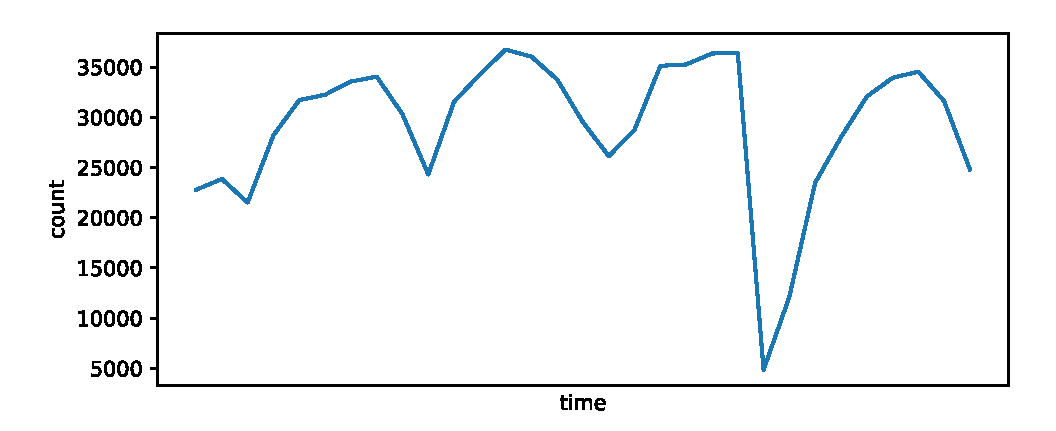
\includegraphics[width=0.9\columnwidth]{images/yellowdata_count.eps}
	\caption{Avg. \# of yellow cab trips for January 2016}
	\label{fig:yellowstats}
\end{figure}
%When we analyze data, we might make some observations that pique our curiosity. We might want to explain trends or anomalies in data.
%Without an automated system, a data analyst has to go through several manual operations to find an explanation. For small datasets, doing so might seem reasonable. 
The tedious task of finding an {\explanation} by manually scraping the data becomes even impossible with big data (e.g., NYC taxi trips).
%However, if we are dealing with a large amount of data like the NYC taxi dataset, manually finding explanations can become a tedious (or even impossible) task.% Our system is designed to produce explanations based on observations over a large amount of data. % In the past few years there has been a lot of developments in the area of Big Data.



% Since existing techniques are designed for non-spatial data, we propose a new approach for explaining spatially heterogeneous data. Our approach expands on the aggravation and intervention techniques while using spatial partitioning/clustering to improve explanations for spatial data. Experiments show that the proposed approach outperforms aggravation in precision and recall while outperforming intervention in precision when finding explanations for observations made on a real NYC taxi dataset as well as a  disease outbreak datasets.

%While some data observations might be interesting, in order to make decisions based on these observations, one might find it useful to find an explanation. For example, someone looking to start a business might look for spatial locations in which their specific category of business succeeds. It might be even more beneficial to find out why it prospers in that specific location.

%We can find several examples of decisions being made using big data analysis in everyday situations. Companies like Uber and Facebook handle large amounts of spatial data every day. Such data can be used to improve service. 
%UPS is saving millions of gallons of fuel per year using big data analytics. UPS uses On-Road Integrated Optimization and Navigation system(ORION) to determine the order of delivery, routes, and loading plans~\cite{upsarticle}.




%Given the tremendous benefits of automated analysis, the motivation for this paper was to create an automated system to help analysts answer questions about observations. The idea is to create a system which works on spatial data in general. This paper comes up with a generic system to explain observations on spatial data.




% For example, if we have taxi cab data, we might want to use this data to figure out the best locations for taxicab stands. Good locations for taxicab stands can result in less fuel consumption and lower wait times for the customers. A similar case can be made for medical emergencies and hospital locations. Even though the cost of building a hospital is much higher than that of building a taxi station, the initial cost of building the infrastructure is assuaged over time if the location is beneficial. Companies like



% In this paper, we look at different approaches to explain these types of observations. In fact, we also look at observations with a spatial dimension.

In this paper, we describe a system that automatically generates potential {\explanation}s to {\fact}s extracted from mobility datasets. The proposed approach takes two types of inputs. One of the inputs is the mobility dataset we want to analyze. The second input is the {\fact} observed by the data scientist. The {\fact} can be in the form of a set of aggregate queries executed on a spatial database. 
%To produce spatial explanations, the system uses one of several different solutions to find an explanation depending on what the user wants. The output of our system is an explanation for our system based on predicates.
The {\explanation}s produced by the system are parts of the data that have a significant effect on what the {\fact} data scientist is observing. %For example, assume the analyst is observing tips (given by customers in each taxi ride) for taxi trips. If removing a few tuples from the dataset has a significant impact on the average tip, then such few tuples would be considered as a potential explanation for the observation. 
Another definition of {\explanation}s in our proposed solution involves looking at different parts of the data. 
%For example, if we divide our data into a number of parts, the parts which deviate from the average value of tip percentage are considered as explanations because they introduce the largest differences.
%In this paper we extend several approaches and compare them. 
%There are three major contributions in this paper:
%\begin{itemize}


There has previously been some work related to database explanations. 
%as well as spatial analytics. 
%Since our automated framework leverages distributed computation frameworks, this section also elaborates the corresponding field. 
%The work by \cite{meliou2010causality} is a survey which looks at causality from a database perspective. Traditionally, work on causality from a database perspective mainly deals with provenance i.e. events which occurred chronologically. 
%This solution, however, only works with databases with timestamps. The paper also looks at the degree of responsibility which is defined as the number of tuples which have to be removed to change a binary observation. An example of a binary observation is winning and losing an election for instance. If a candidate wins by a high margin, each tuple has a lower degree of responsibility. On the other hand, a close victory for a candidate increases each voters degree of responsibility. 
Existing works on causality and {\explanation}s in both the Artificial Intelligence and Database communities are summarized in~\cite{meliou2014causality}. It turns out that AI problems tend to have a bigger causal network while database problems tend to have more variables.
There has also been a lot of work on correlation which shares some common ground with the work on explanations. One interesting recent work on the subject is the Data Polygamy framework \cite{chirigati2016data}. This framework is designed to find the correlation between a corpus of datasets. It uses the peaks and troughs of the data to calculate \textit{salient features} \cite{dunn1986applied}. The positive and negative correlation between these salient features can be used to decide whether datasets are related\cite{su2014supporting}. The objective of our system is a bit different from finding correlations. There are a number of different factors which can affect {\fact}s. Correlation might be one of these attributes in certain cases. But if we ignore other criteria, such as selectivity, we might get results that do not have a significant impact. For example, if two attributes are highly correlated in a certain spatial cluster but the selectivity of the cluster is high, it would lead to a low impact on the {\fact}.




%\item We extend aggravation and intervention for spatial explanations/observations. Aggravation and Intervention techniques in literature are designed for giving non-spatial explanations for non-spatial observation. When we look at spatially heterogeneous data, the spatial context has an impact on the value of the explanations.

% \item We extend the use of salient features to give spatial explanations for simple observations based on attributes. Salient Features can be used to compare the correlation between attributes between multiple datasets. However, we repurpose the use of salient features for explanations. We use the salient features for attributes in the same dataset to form explanations.

%\item 
In this paper, we introduce a new approach: {\solution}, which employs a spatial partitioning/clustering technique to find spatial explanations for spatially heterogeneous data. Our solution is inspired by the work \cite{roy2014formal}, which outlines a formal approach to explain data. The main solutions outlined in that work are Aggravation and Intervention. However, the work in \cite{roy2014formal} is designed to work with non-spatial datasets. One of the main points of the paper is that their approach works on a dataset which can span several tables related by primary and foreign keys. While the approach is great for non-spatial data, it does not translate well in the spatial domain. 
%This approach develops on previous work in causality and influence. 
It also resembles data mining concepts related to association rule mining \cite{agarwal1994fast,tan2006introduction}. 
%In association rule mining sets of attributes that occur together are assigned support and confidence. The support measures the frequency of occurrence of a set of attributes while confidence measures how frequently an attribute occurs with another set of attributes. The work by \cite{koperski1995discovery} looks at association rule mining in a spatial context. Given a set of spatial relationships, it applies association rule mining to find relationships that frequently occur together. 
There is a difference between association rule mining and our proposed approach. First of all, our proposed approach uses a user-defined observation. Secondly, in our approach, we are not looking at the associations but rather at the effect of removing or filtering pieces of data. A high association between predicates does not necessarily mean that removing them will significantly affect the {\fact}.


%for different dimensions of spatial explanations. Therefore, we propose a new approach which uses a spatial hierarchy. This accounts for explanations for multiple dimensions of the data.
%\item 
We introduce a method to balance influence and intensity to give better {\explanation}s. Influence and Intensity measure the global and local impact of an explanation, respectively. We acknowledge that the user of our system can have a non-binary preference for either. We construct our system in a way that it produces explanations as a linear relationship between influence and intensity.
%\item 
%We introduce an automated system for giving explanations based on our findings. The system that we have defined has a lot of parameters. It requires observations, coefficients, arithmetic relationships and selectivities as parameters.
%\end{itemize}


% In this thesis we define a taxonomy(Section~\ref{sec:taxonomy}) for observations and explanations.  The observation we made in Fig.\ref{fig:yellowstats} can be considered as a non spatial observation. Its explanation can either be non spatial or spatial. The first class in our taxonomy deals with non spatial explanations for non spatial observations(Section~\ref{sec:nonspatial_nonspatial}). The second class is related to spatial explanations for non spatial observations(Section~\ref{sec:spatial_nonspatial}) while the last class is about spatial explanations for spatial observations. Many geospatial datasets that we encounter contain time as one of the attributes. When we talk about spatial explanations, we do not take time into consideration. Instead, time is considered as a non-spatial attribute.

% There are three main approaches to explanation that we study in this thesis. Each approach has been extended to satisfy our taxonomy. Each approach relies on the fact that the observation is an aggregated attribute in our data set while the explanation is a predicate. \textbf{Aggravation}(Section~\ref{sec:aggravation}) is based on the principle that if we consider only the tuples in our database satisfying our explanation predicate, the value of the observation on our modified dataset will be our measure of aggravation\cite{roy2014formal,meliou2014causality}.

% In contrast, \textbf{Intervention}(Section~\ref{sec:intervention}) measures the influence of our explanation i.e. what will be the value of our observation when all the tuples satisfying our explanation predicate are removed\cite{roy2014formal}. We also extend Intervention to introduce \textbf{Hierarchical Intervention}(Section~\ref{sec:hei_intervention}). This approach measures the value of intervention when the explanation consists of a cluster of spatial polygons in our explanation predicate.

% Finally, \textbf{Salient Features}(Section~\ref{sec:salient_features}) can be used to find explanations\cite{chirigati2016data}. Each salient feature encapsulates a polygon where an attribute in the dataset is pronounced. The correlation between a salient feature of the observation and the salient feature of the explanation can give us possible explanations.

% Each approach has its own set of advantages and disadvantages. While one approach might give us very specific explanations that show a textbook example of our observation, another might give us an explanation which is hard to see in the context of the observation but has a large overall impact on it. One of the objectives of this paper is to compare which approach is suitable considering its context.

% We implemented(Section~\ref{sec:implementation}) these approaches, including hierarchical intervention using distributed data frameworks\cite{borthakur2007hadoop,dean2008mapreduce,shanahan2015large,zaharia2016apache}. We made optimizations in our implementation to make sure our approach is orders of magnitude faster than the naive approach. The implementation of salient features was used from the Data Polygamy framework \cite{chirigati2016data}.
% In order to compare each approach, we defined a few evaluation metrics. The \textbf{Intensity}(Section~\ref{sec:intensity}) metric measures how relevant each explanation is to the observation. To be more specific, it measures the value of the observation for the top explanations for each approach. The \textbf{Influence}(Section~\ref{sec:influence}) metric measures the observation when the top explanation is removed from the data. We also compare the speed(Section~\ref{sec:speed}) of our implementations of each approach.



% The approaches that we mention in his paper borrow from previous work on explanation and correlation. We have extended existing frameworks to work on our specific taxonomy. Aggravation(Section~\ref{sec:aggravation}) and Intervention(Section~\ref{sec:intervention}), for instance, are approaches which are originally designed to work in a non spatial context. They provide explanations in the form predicates over attributes. If we have a dataset with latitude and longitude as the spatial attributes, they may provide explanation in terms of just a latitude or longitude as separate continuous attributes. They might even provide explanations with no spatial attributes at all. Another drawback of using these approaches with spatial data is that they function without any knowledge of spatial locality.
%
% We highlight a new approach called hierarchical intervention (Section~\ref{sec:hei_intervention}). This approach intends to use clusters of spatially co located points or polygons in an attempt to come up with better explanations. As the name suggests, this approach borrows from the intervention approach. It uses spatial partitioning to improve spatial explanations.
%
% Another contribution of this paper is outlining a method for using salient features for explanations. The salient features approach is originally intended to work for correlation between datasets. Our extension of this approach intends to use it for the purpose of explanations. Extending salient features for explanation rather than correlation involves some additional step of work while discarding parts of the previous work which relates specifically to correlation. The original work uses salient features to compare multiple datasets and rank the most correlated datasets. Our usage of salient features is intended to explain only a single dataset with multiple attributes. Even if two attributes of a dataset are highly correlated, it may or may not rank the two attributes in the top explanations depending on the observation.

%We compare the different approaches in this paper. In order for us to compare different things, we need to do so on the basis of a common standard. The different solutions to the explanation problem are structurally very different from each other. As previously mentioned, some of them are originally not designed to handle spatial data. We have designed a common taxonomy to compare all these different solutions. On top of designing this taxonomy, our extension of each approach is designed to make sure each solution adheres to the taxonomy. Even though, this still leaves room for differences between each solution, it gives us room for comparison.

%We also define a number of evaluation metrics and an approach which uses them to come up with better explanations.

%\section{Related Work}
There has previously been some work related to database explanations as well as spatial analytics. 
In this section, we elaborate on the existing in such a field of study. 
%Since our automated framework leverages distributed computation frameworks, this section also elaborates the corresponding field.% Most of this work revolves around the notion of causality. There is existing work in the field of Artificial Intelligence by \cite{zhang2002discovering} which expresses relationships between different attributes in a dataset as conditional probabilities. Based on the conditional probability each tuple is given a set of binary rankings.

{\bf Causality in databases.} The work by \cite{meliou2010causality} is a survey which looks at causality from the perspective of a database problem. Traditionally, work on causality from the database perspective mainly deals with provenance i.e. events which occurred chronologically. This solution, however, only works with databases with timestamps. This paper also looks at the degree of responsibility which is defined as the number of tuples which have to be removed to change a binary observation. An example of a binary observation is winning and losing an election for instance. If a candidate wins by a high margin, each tuple has a lower degree of responsibility. On the other hand, a close victory for a candidate increases each voters degree of responsibility. The paper by \cite{meliou2014causality} is a survey of work in causality and explanations in both the Artificial Intelligence and Database communities. The take away from this survey is that AI problems tend to have a bigger causal network while database problems tend to have more variables.

{\bf Salient features correlation.} There has also been a lot of work on correlation which shares some common ground with the work on explanations. One interesting recent work on the subject is the Data Polygamy framework \cite{chirigati2016data}. This framework is designed to find the correlation between a corpus of datasets. It uses the peaks and troughs of the data to calculate \textit{salient features} \cite{dunn1986applied}. The positive and negative correlation between these salient features can be used to decide whether dataset are related \cite{su2014supporting}. 
%The objective of our system is a bit different from finding correlations. 
However, there are a number of different factors which can affect observations and correlation is only one of these attributes in certain cases. 
If we ignore other criteria such as selectivity then we might get results which do not have a significant impact. E.g. if two attributes are highly correlated in a certain spatial cluster but the selectivity of the cluster is small, it would lead to a low impact on the observation.

%{\bf Why not explanation} There has also been work related to why not explanations in databases. The work by \cite{ten2015high} looks at the question of why some tuples are missing from database results. This paper uses the assumption that the relationship between tuples is defined in the form of an ontology. The paper uses the relationship between the ontology for a schema and the ontology for an instance of the schema to judge whether an explanation exists. The ontologies that are used can be created manually or automatically. Using provenance \cite{cheney2009provenance} can help in creating ontologies.

{\bf Aggregation and intervention.} 
%Our solution mainly builds upon work by \cite{roy2014formal} which outlines a formal approach to explain data. 
The main solutions outlined in \cite{roy2014formal} are Aggravation and Intervention. 
It formally defines the {\fact} and {\explanation} in the problem of data explanation. 
The predicates on different attributes of the central table are exploited as the candidate {\explanation}s.
{\aggravation} and {\intervention} are defined based on the {\explanation} itself and the remaining data respectively. 
However, it is designed to work with non-spatial datasets. 
This method ignores the impact and characteristics of spatial data. 
So it does not translate well in the spatial domain and cannot find meaningful spatial {\explanation}s.
%One of the main points of the paper is that their approach works on a dataset which can span several tables related by primary and foreign keys. 
%While the approach outlined by \cite{roy2014formal} is great for non-spatial data, it does not translate well in the spatial domain. 
%This approach develops on previous work in causality and influence. It also resembles data mining concepts related to association rule mining \cite{agarwal1994fast,tan2006introduction}. 
%In association rule mining sets of attributes that occur together are assigned support and confidence. The support measures the frequency of occurrence of a set of attributes while confidence measures how frequently an attribute occurs with another set of attributes. The work by \cite{koperski1995discovery} looks at association rule mining in a spatial context. Given a set of spatial relationships, it applies association rule mining to find relationships that frequently occur together. There is a difference between association rule mining and our proposed approach. First of all, our proposed approach uses a user-defined observation. Secondly, in our approach, we are not looking at the associations but rather at the effect of removing or filtering pieces of data. A high association between predicates does not necessarily mean that removing them will significantly affect the observation.

%{\bf Spatial regression.} Spatial regression techniques can be used to explain data \cite{dunn1986applied,cleveland1988locally}. The idea behind regression techniques is to express an attribute that we are interested in as a dependent variable. This dependent variable can then be expressed in the form of a parametric equation involving other attributes in the dataset as independent variables. The user of this system decides a dependent variable and a set of explanation variables. The resulting equation has coefficients assigned to each explanatory variable as well as a bias term. This results in a curve fitting problem. The curve fitting problem is solved using regression i.e. the coefficient terms and the bias are iteratively adjusted until the sum of squared error between the predicted curve and the ground truth results in a minimum value. Regression techniques are widely used for spatial data analysis. However, they depend on predefined spatial partitioning and look at the data as a whole rather than from the perspective of a user-defined observation.
% Geographically Weighted Regression(GWR) expands on OLS regression for geospatial data \cite{brunsdon1998geographically,charlton2009geographically}. GWR tries to use the regression equation for each feature in the dataset. It uses the idea that spatially co-located points contribute more to each other by using a spatially aware kernel function. A kernel function like a Gaussian, for example, gives more weight to nearby points than to points which are far apart.

%{\bf Spatial autocorrelation.} Besides work related to explanation, there has been a lot of research in the area of spatial correlation. Much of the work in this area extends from multiple old works by Getis \cite{getis1991spatial,ord1995local,getis1996local,getis2002comparative,getis2007reflections}. The Getis Ord statistic \cite{ord1995local} for example is useful in showing us areas with high local spatial associations. The Moran's I statistic is useful for measuring the spatial heterogeneity of the data \cite{assuncao1999new,zhang2008use}. Moran's I is useful in hot spot analysis which can be viewed as a step in the way of finding explanations.


%\section{Big Spatial Data Systems.}
%{\bf Distributed data systems} Map Reduce \cite{dean2008mapreduce} is a framework for data processing which is designed for taking distributed and parallel computation into perspective. There are three main operations in a MapReduce process: map, shuffle and reduce. The map operation assigns a key to each element and performs any necessary transformations. The shuffle operation relocates the elements such that elements with the same key are nearby(since they are going to need each other in calculations). The reduce step performs a calculation on each element with the same key and returns the output. Spark \cite{shanahan2015large,zaharia2016apache} is a distributed and parallel processing framework. Spark uses a directed acyclic graph to perform calculations. Since the DAG created by Spark can have a lot of common nodes between tasks, the computational complexity of the operation is reduced compared to MapReduce.
%Geospark~ \cite{yu2015geospark} is a framework for performing several spatial operations on data in Apache Spark. It also has a component which helps in data visualizations \cite{yu2018src}.
\section{System Overview}
%\section{Star Schema}
%{\bf Star Schema.} 
%{\bf Star schema.} 

Figure~\ref{fig:framework} shows the system diagram for our solution which uses hierarchical intervention. 
The back-end of the system is the spatial data and a spatial database system. 
Users may discover observations by searching the data. Their observations can be generated from data histograms and aggregated queries.
%We take inputs in the form for aggregate queries. An arithmetic expression encapsulates the relationships between these queries. 
The partitioner create a hierarchy partitions on top of spatial data. Depending on the hierarchy that we have created and our inputs, we perform aggravation and intervention. The results of aggravation and intervention are used to in a ranking system based on an explanation index. The explanation index evaluator measures the quality of candidate explanations and outputs the top-k explanations. 
%How much each explanation approach is weighted in the explanation index is under the control of the data analyst. 
%Finally, the top results are used for visualization. We have created a web-based GUI to display these kinds of explanations.

\begin{figure}[t]
	\centering
		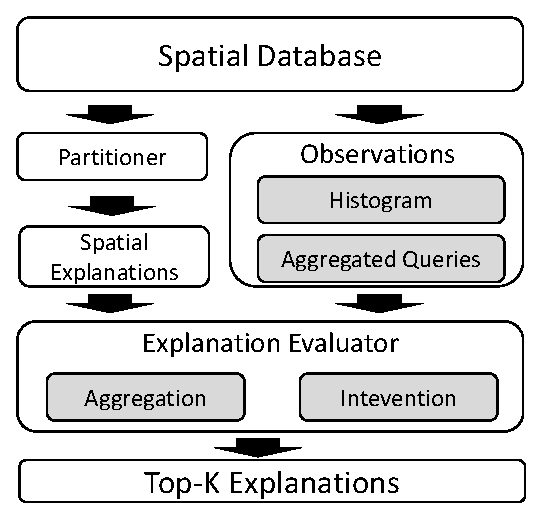
\includegraphics[width=0.4\textwidth]{images/architecture.eps}
		\caption{An outline for our system framework}
	\label{fig:framework}
\end{figure}

The proposed system has the underlying assumption that the data that will be used to generate explanations is the Fact Table for a Star schema\cite{giovinazzo2000object,adamson2010star}. To understand the Fact Table, it is important to understand the structure of the Star Schema. A traditional relational database system contains a set of tables related by primary and foreign keys. For instance, we can use our running example of the NYC Taxi Trips dataset to illustrate a Star Schema. The trips and payment type can be represented in separate tables. One trip can have a single payment type while a payment type can be used in multiple trips. This is an example of a one-to-many relationship.
In order to represent this data in a relational database, the $trips$ table and the $payment\_type$ table need to have a primary and foreign key. Table~\ref{tbl:fact} can be considered as the central part of the schema because it contains the foreign key to the $payment\_type$ table.



% \begin{center}
% \small
%   \begin{tabular}{ | l | c | }
%     \hline
%     \textbf{PaymentTypeId} & \textbf{Name} \\ \hline
%     1 & Credit Card  \\ \hline
%     2 & Cash  \\ \hline
%     3 & No Charge  \\
%     \hline
%   \end{tabular}
% \end{center}
% \captionof{table}{Payment Type Table}
% \label{tbl:payment_type}

% \begin{center}
%   \begin{tabular}{ | l | c | r | }
%     \hline
%     \textbf{StudentId} & \textbf{Name} & \textbf{Grade} \\ \hline
%     1 & John Doe & 3.2 \\ \hline
%     2 & Alice & 3.3 \\ \hline
%     3 & Bob & 3.8 \\
%     \hline
%   \end{tabular}
% \end{center}
% \captionof{table}{Students Table}
% \label{tbl:student}

\begin{center}
\small
  \begin{tabular}{ | l | l | c | l | }
    \hline
    \textbf{pickup\_lat} & \textbf{pickup\_lng} & \textbf{PaymentType} & \textbf{tip\_percentage} \\ \hline
    34.4 & -74.2 & 1 & 15.3 \\ \hline
    34.6 & -74.1 & 1 & 10.2 \\ \hline
    34.6 & -74.3 & 1 & 9.8 \\ \hline
    34.8 & -74.6 & 2 & 11.2 \\ \hline
    34.6 & -74.3 & 1 & 10.7 \\ \hline
    34.9 & -74.1 & 3 & 0.0 \\
    \hline
  \end{tabular}
\end{center}
\captionof{table}{\small Trips Table. PaymentType 1, 2, and 4 represent Credit Card, Cash, and No Charge, respectively.}
\label{tbl:fact}

This type of schema where there is a central table consisting of facts while the remaining tables contain the meta data is called a star schema. The central table is called the Fact Table, whereas, the tables containing the meta data are called the Dimension Tables (such as the payment type table in the NYC Taxi Trip dataset).% In the case of the schema we just defined, Table.~\ref{tbl:payment_type} is the dimension table while Table.~\ref{tbl:fact} is the fact table.

%\section{Observations}
% \begin{figure}[ht]
%   \begin{center}
%   \includegraphics[width=0.5\columnwidth]{observationexample}
%   \end{center}

%   \caption{An histogram showing an example observation}
%   \label{fig:observation_example}
% \end{figure}

{\bf Numeric Query.} A numeric query is an expression of the form:
$$Q = E(q_1, q_2, .., q_m)$$
Here $q_i$ is any SQL query which contains an aggregate function. The aggregate function can be SUM, COUNT, and AVERAGE. So each $q_i$ will return a single numeric value. $E$ represents a numeric expression based on the result of $q_1$, $q_2$, .., $q_m$. The operator in $E$ can be any numeric operator, such as $+$, $-$, $*$, $/$, $log$, etc.

{\bf {\Fact}.} A {\fact} is a pair $(Q, dir)$, where (1) $Q$ is a numeric query, (2) $dir \in \{high, low\}$ is direction indicating whether the user thinks $Q$ is higher or lower than the expected value.

{\bf Example.} In Figure \ref{fig:spatial_explanation_example}, there a {\fact} that the number of taxi trips in NYC on January 23, 2016 dropped drastically. Such {\fact} can be represented by two queries, $q_1$ and $q_2$ as follows:

\renewcommand{\lstlistingname}{Query}% Listing -> Algorithm
\begin{lstlisting}[language=SQL, caption=Aggregate Query for the number of taxi trips on January 22, label=qry:aggregateexample1]
SELECT COUNT(*) FROM
FROM nyc_data
WHERE date = 'January 22, 2016'
\end{lstlisting}
\renewcommand{\lstlistingname}{Query}% Listing -> Algorithm
\begin{lstlisting}[language=SQL, caption=Aggregate Query for the number of taxi trips on January 23, label=qry:aggregateexample2]
SELECT COUNT(*) FROM
FROM nyc_data
WHERE date = 'January 23, 2016'
\end{lstlisting}
The difference in the number of taxi trips between the two dates can be represented by a numeric query $Q = \frac{q_1}{q_2}$. The number of taxi trips drops drastically, so it means the value of $Q$ is lower than the expected value. Then the {\fact} has the format $(\frac{q_1}{q_2}, low)$.

When a table is analyzed, users may find an interesting {\fact} from the data table. This {\fact} is issued to the system with the defined format as the input. Then the system will try to find out the {\explanation} for the {\fact}.

%{\bf {\Fact}s.} {\Fact}s are features in the data that the user wants to explain. {\Fact}s are defined as arithmetic expressions over a set of aggregate queries. Let $F$ be the fact table in our star schema dataset. In the course of this document, we will be using relational algebra expressions defined by \cite{elmasri2011fundamentals} for aggregate expressions. Thus, the $\mathscr{F}$ symbol represents an aggregate function. An aggregate query is defined as:
%$$_A\mathscr{F}_B(D), A \in F$$
%$B$ is an aggregate function. $A$ is an attribute in our dataset. $D$ is the fact table. Examples of an aggregate function include SUM, COUNT, and AVERAGE.
%We use SQL to construct an example for an observation. Queries~\ref{qry:aggregateexample1} and \ref{qry:aggregateexample2} show examples of aggregate queries.

% Observations made on data can also be represented on histograms. Fig.~\ref{fig:observation_example} shows an example of an observation. The green bar on the histogram represents an aggregate query where the day is Friday.

%\renewcommand{\lstlistingname}{Query}% Listing -> Algorithm
%\begin{lstlisting}[language=SQL, caption=Aggregate Query for average tip percentage with credit cards, label=qry:aggregateexample1]
%SELECT AVG(tip_percentage) FROM
%FROM nyc_data
%WHERE payment_type = 1
%\end{lstlisting}
%\renewcommand{\lstlistingname}{Query}% Listing -> Algorithm
%\begin{lstlisting}[language=SQL, caption=Aggregate Query for average tip percentage with cash, label=qry:aggregateexample2]
%SELECT AVG(tip_percentage) FROM
%FROM nyc_data
%WHERE payment_type = 2
%\end{lstlisting}

%Using these aggregate queries we may form an observation based on the ratio of tip percentage with credit card against tip percentage with cash.
%$$observation = \frac{\textnormal{Query.~\ref{qry:aggregateexample1}}}{\textnormal{Query.~\ref{qry:aggregateexample2}}}$$


%\section{Explanations}
{\bf {\Explanation}.} We represent an {\explanation} as a predicate $\phi$. 
A predicate $\phi$ is a conditional statement which results in a boolean value. An {\explanation} indicates a set of tuples in the data table which satisfy the predicate. For non-spatial {\explanation}, $\phi$ has the format of $[A$ $op$ $c]$, where $A$ is an attribute in the data table, $op$ can be $=$, $<$, $\leq$, $>$, $\leq$ and $c$ is a numeric value. For example, we can have an non-spatial {\explanation} as follows:
$$\phi: PaymentType = 1$$
If we use such {\explanation} to explain the {\fact} mentioned previously, it means we think that the drop on 22 January, 2016 is caused by the trips which are paid by Type 1 (but actually this explanation does not make sense).

%We go into more details for the formal definition of different kinds of explanations in Section~\ref{sec:taxonomy}. 
%If we consider Queries~\ref{qry:aggregateexample1} and \ref{qry:aggregateexample2} as an example. The explanation would be in the form of a predicate:
%$$tip\_percentage = 15.3$$
%
%Let $D$ be our solution space. We can define our predicate to be the function $P$. Let $X$ represent a set of attributes in our schema. Our explanation can now be formally defined as:
%
%\begin{equation}
%X|P(X):=
%    \begin{cases}
%      \text{true}, & \text{if}\ X \in D \\
%      \text{false}, & \text{otherwise}
%    \end{cases}
%\end{equation}

%Note that $P$ is an open ended function. In the case of spatial explanations, $P$ can take the form of a spatial function like $ST\_CONTAINS$ in PostGIS i.e. whether a polygon contains a point. In the non spatial context, $P$ can represent functions like 'greater than', 'less than', etc.


{\bf {Explanation via Intervention.}} 
%\my{Intervention is an approach inspired by the concept of influence. It builds on the \my{aggravation} approach(Section~\ref{sec:aggravation}).}  
The Intervention approach measures how much the {\fact} would change had the explanation not been present. Let $D$ be the dataset we are interested in and $Q$ be a function which returns the value of our target {\fact} given a dataset. Keeping our taxonomy in context, this means $Q$ returns the value of our aggregate {\fact} query. Denote $\phi$ as one candidate {\explanation}. Let $\Delta_\phi \leftarrow \sigma_\phi(D)$ be a subset of $D$ that satisfy $\phi$. Then $D - \Delta_\phi$ represents the remaining part after removing $\Delta_\phi$ from $D$. The direction of the {\fact} can either be \textit{high} or \textit{low} depending on whether we are interested in the greatest or least values of {\fact} respectively. Given a dataset $D$, a {\fact}$(Q, dir)$, the degree of an {\explanation} $\phi$ by intervention can be defined as follows:
\begin{equation}
\delta_{int}:=
\begin{cases}
-Q(D-D_{\phi}), & \text{if}\ direction=high \\
Q(D-D_{\phi}), & \text{otherwise}
\end{cases}
\end{equation}

The degree of candidate explanation by intervention must be higher the closer we are to the direction of the observation, therefore, we use the negative value when the direction is high. If the influence of the candidate explanation is high, it will result in a low observation value once the candidate explanation is removed from the dataset.
Since intervention extends the idea presented by aggravation, it has similar issues when it comes to the number of permutations for candidate explanations. Similar to our approach in aggravation(Section~\ref{sec:aggravation}), we can reduce the number of permutations by \my{bucketing} the attributes. We can extend intervention for spatial observations and explanations the same way we did for aggravation. The set $P$ consists of distinct non overlapping polygons in our dataset $D$. Let $s$,$t$ be the spatial attributes in $D$. \my{Each tuple in $P$ has two attributes: $polygon\_id$, and $polygon$.}


{\bf Finding Spatial Explanations.}
%{\bf Spatial {\Explanation}.} 
A spatial {\explanation} is different that general {\explanation} in that it is represented by a spatial predicate. A spatial {\explanation} actually indicates a set of data tuples that can satisfy the spatial predicate. We denote a spatial {\explanation} as $\phi_S$.
Spatial explanations take the spatial attributes of the data into consideration. In contrast to non spatial explanations, the candidate spatial explanations consists of polygons. Since we base our proposed approach on the assumption that important tuples are spatially co-located, points which fall inside these polygons form a candidate explanation. 
%Let $S$ be the spatial attributes of $D$ and $P$ be the set of all possible polygons that can be formed from $S$. Let $G$ be a function such that$G(s,t)$ is true when $(s,t) \in P$ and false otherwise, where $s$,$t$ are the dimensions of a point in the Cartesian plane. Our candidate explanation can be defined as,
%$$\phi  \models \vee_{l,k} G(l,k)$$
%where $k,l \in A_D$

%\my{This example should be modified because it looks like a non-spatial explanation.}
%To illustrate spatial explanation in action, we can use NYC TLC data again. Fig.~\ref{fig:spatial_explanation_example} shows the explanation in terms of tip percentage where the observation is also the average tip percentage.

%\begin{figure}[ht]
%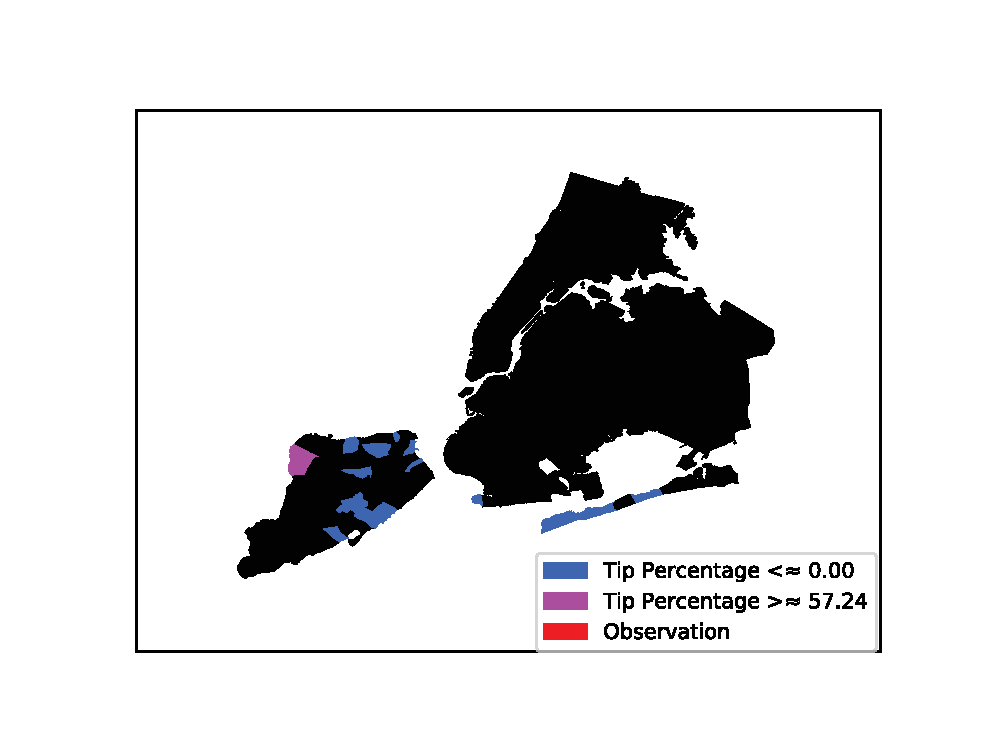
\includegraphics[width=\columnwidth]{images/spatial_explanation_example.eps}
%\caption{An example of spatial explanation}
%\label{fig:spatial_explanation_example}
%\end{figure}

The polygons painted purple show polygons in the candidate {\explanation} where the tip percentage is high, while polygons painted blue show candidate explanations where the tip percentage is low. It should be noted that $P$ has a high number of permutations. It is up to the approach to decide which polygons to include in the candidate explanation. For instance, hierarchical intervention may choose polygons in a spatial proximity while aggravation may choose otherwise.
\begin{figure}[t]
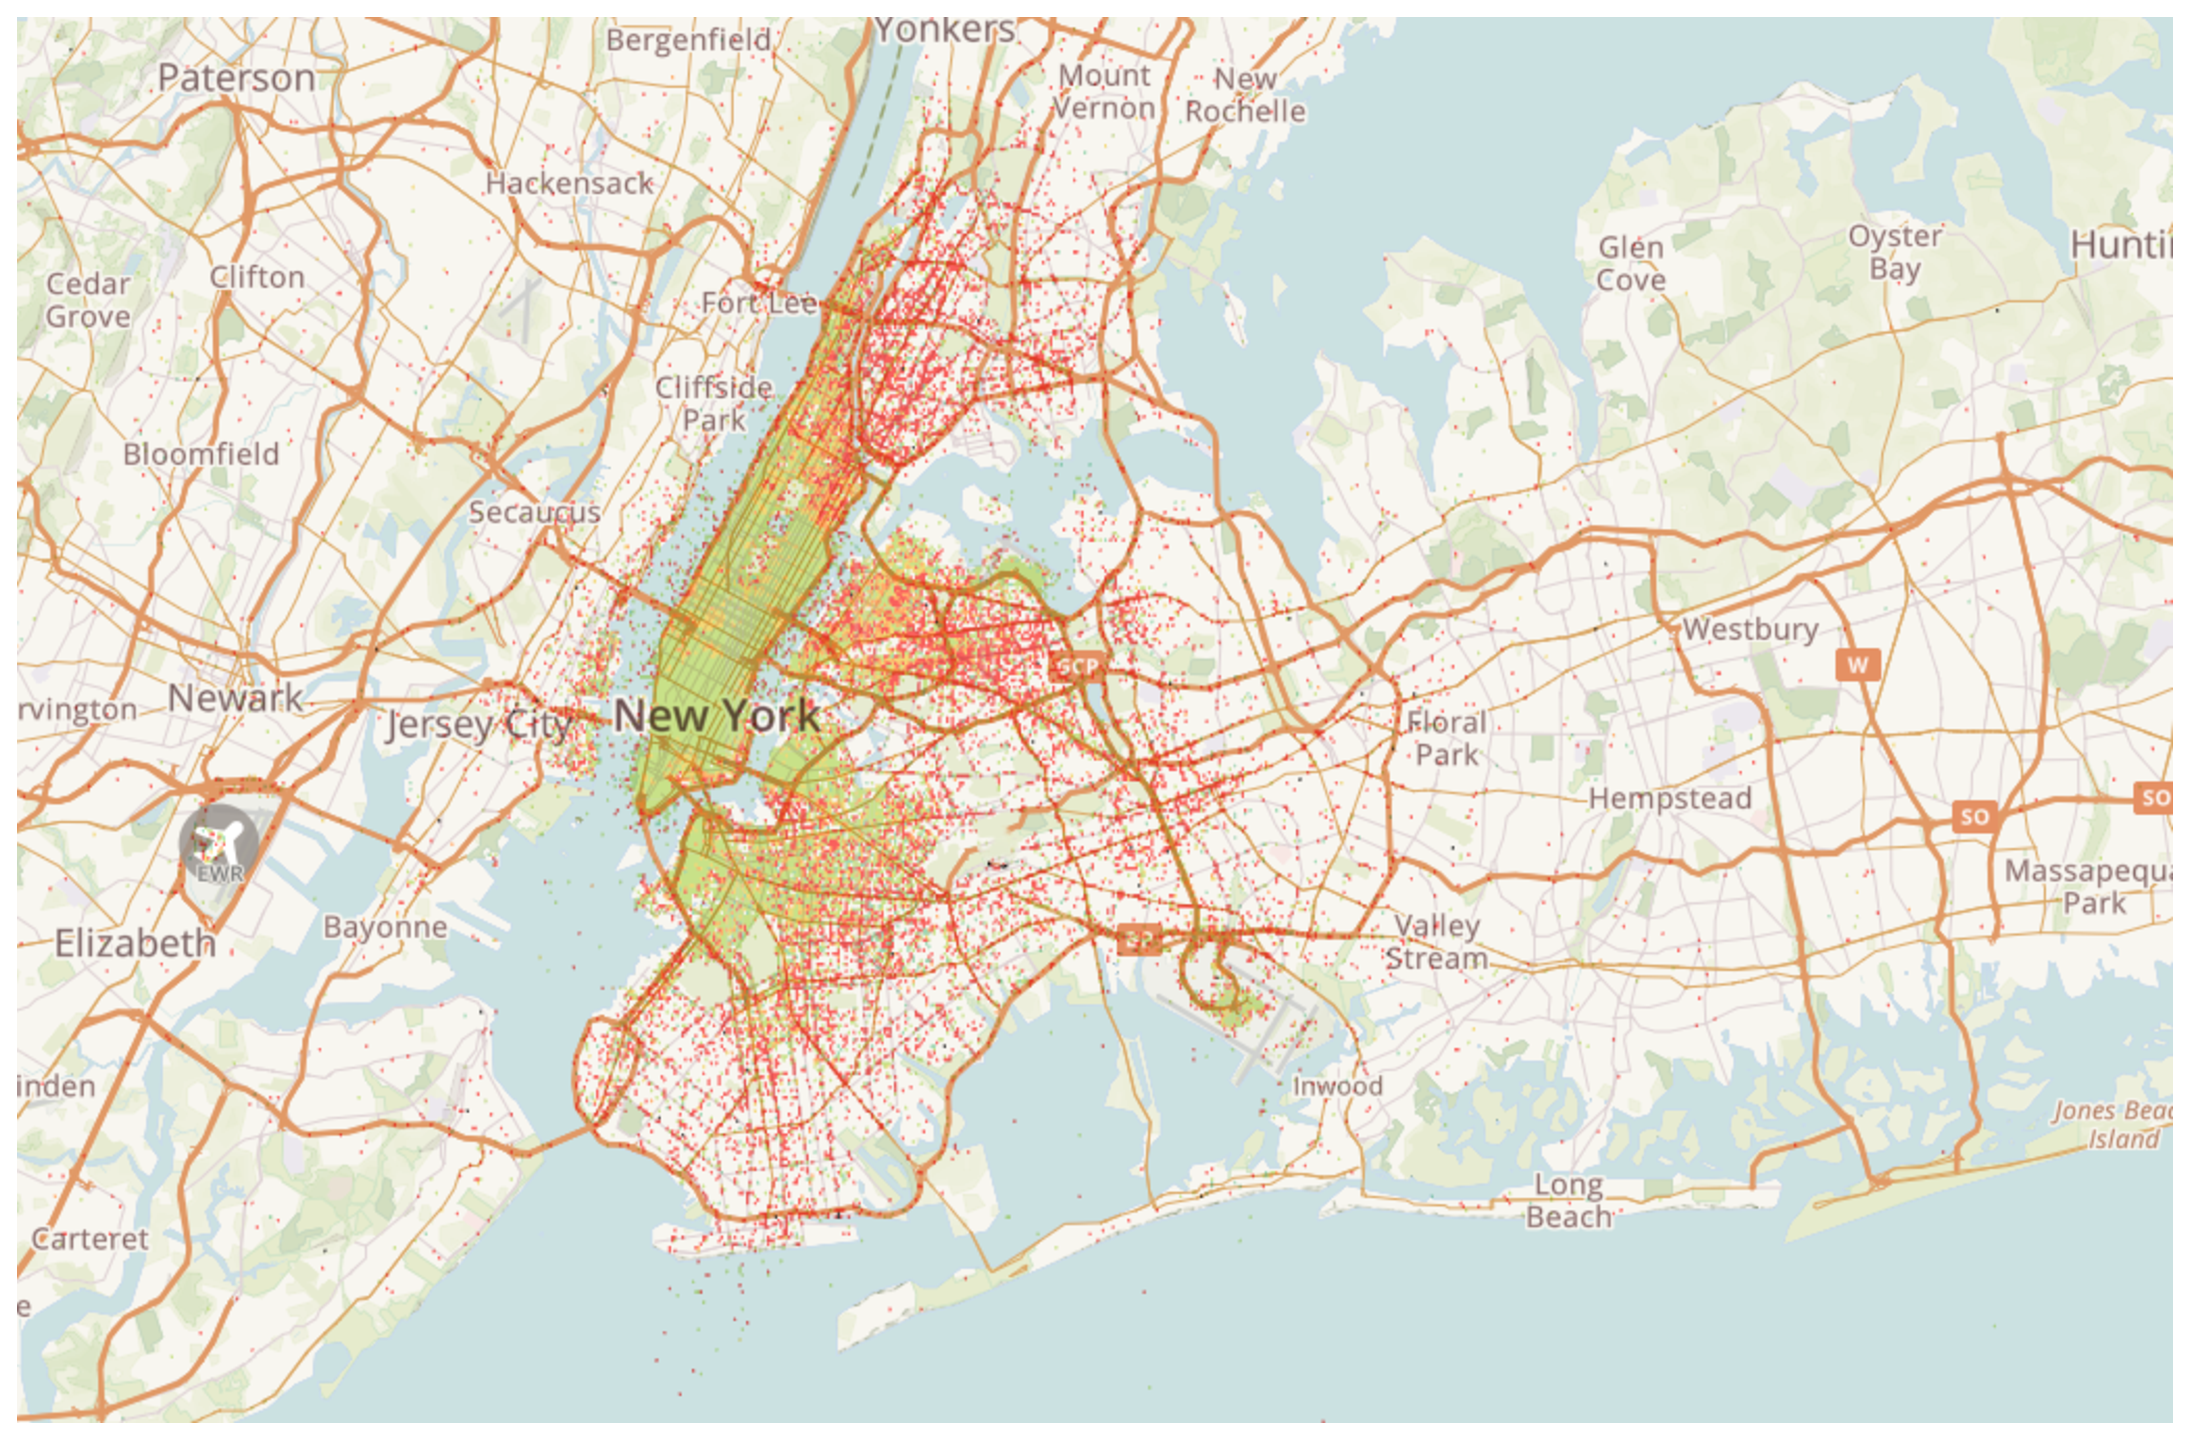
\includegraphics[width=\columnwidth]{images/scatter}
\caption{Heatmap for NYC trips for January 2016}
\label{fig:square_unit_grid}
\end{figure}

\my{Another interesting consideration when we are talking about spatial explanations is the density of the data. Fig.~\ref{fig:square_unit_grid} shows the heatmap for tip percentage with respect to pickup coordinates. It is interesting to observe that the explanations provided in Fig.~\ref{fig:spatial_explanation_example} are all areas with low density of data. One of the reasons for this is because each approach takes some liberty with our definition of the taxonomy. Even though, we defined $P$ to contain all permutations of polygons, an approach may use limited polygons, such as neighborhoods or zones. The way the explanation is ranked also plays a large role.}




% \section{Front End Visualization Tools}
% React\cite{reactjs} is a front end framework which originated in Facebook. The React framework allows interfaces to be designed using components. Each component has properties and a state. A component can have subcomponents. This makes it simpler to design interfaces which show consistent data across components. Some of the charts included in the interface make use of the eCharts library\cite{echarts}.

% MapBox\cite{mapbox} is a library for displaying maps. The maps provided by mapbox consists of tiles and vectors. Each tile represents a cube of the map while vectors are shapes which represent roads, buildings, etc. Deck.gl\cite{deckgl} is a library for creating an overlay on top of the map. Examples of overlays include scatterplots, cartograms etc. Matplotlib was also used for static plots for evaluation\cite{hunter2007matplotlib}.

% We have used all of these tools in a GUI for our our framework. The details of the implementation can be found in Section~\ref{sec:implementation}

\section{Hierarchical intervention}
\label{sec:hei_intervention}
%\section{System Overview}
%\section{Star Schema}
%{\bf Star Schema.} 
%{\bf Star schema.} 

%\section{Hierarchical intervention}
%\label{sec:hei_intervention}
It is not trivial to generate candidate spatial {\explanation}s. 
Spatial data is continuous in the space, which makes it impossible to naturally divide data into buckets like what we have done for the attribute \emph{PayType}. 
For such type of attribute, one common solution is to partition based on value range. 
This solution makes sense for one-dimensional attribute. 
However, spatial data is continuous in 2-Dimensional space. 
A straight solution to partition data is to use grid cell, which is directly extended from the 1-dimensional's partition based on value range. 
This method suffers from the data skewness, which means that some grid cells are empty while some grid cells are super crowded. 
Another problem is to determine the number of partitions. 
In order to cope with these problems, we propose a solution called {\solution}. 

%\section{Introduction}
%This section details our approach called Hierarchical Intervention which is an extension of the intervention approach. 
The idea behind hierarchical intervention is to improve the generated explanations by grouping spatially co-located polygons in the candidate set of explanations. The whole space is divided into different number of partitions in several levels in pyramid manner. The highest level contains the entire space as one predicate, while each predicate in the lowest level contains one zone or a point.



%\subsection{Intervention approach with spatial support}
%
%Intervention is an approach inspired by the concept of influence. It builds on the aggravation approach(Section~\ref{sec:aggravation}). Intervention tries to measure how much our observations would change had our explanation not been present. Let $D$ be the dataset we are interested in. Let $Q$ be a function which returns the value of our observation given a dataset. Keeping our taxonomy in context, this means $Q$ returns the value of our aggregate observation query. Let $\phi$ be our candidate explanation. Let $\Delta_\phi \leftarrow \sigma_\phi(D)$. Let $D_\phi = D - \Delta_\phi$. The direction of our observation can either be \textit{high} or \textit{low} depending on whether we are interested in the greatest or least values of observation respectively. Our degree of candidate explanation by intervention, $\delta_{int}$, can then be expressed as,
%\begin{equation}
%\delta_{int}:=
%\begin{cases}
%-Q(D_\phi), & \text{if}\ direction=high \\
%Q(D_\phi), & \text{otherwise}
%\end{cases}
%\end{equation}
%
%We want the degree of candidate explanation by intervention to be higher the closer we are to the direction of the observation, therefore, we use the negative value when the direction is high. If the influence of the candidate explanation is high, it will result in a low observation value once the candidate explanation is removed from the dataset.
%
%Since intervention extends the idea presented by aggravation, it has similar issues when it comes to the number of permutations for candidate explanations. Similar to our approach in aggravation(Section~\ref{sec:aggravation}), we can reduce the number of permutations by bucketing the attributes. We can extend intervention for spatial observations and explanations the same way we did for aggravation. The set $P$ consists of distinct non overlapping polygons in our dataset $D$. Let $s$,$t$ be the spatial attributes in $D$. Each tuple in $P$ has two attributes: $polygon\_id$, and $polygon$.

%\subsection{Hierarchical intervention overview}
{\bf Main idea.} The proposed algorithm partitions the data spatially into a hierarchy. 
The top level of the hierarchy consists of all the tuples in the data. 
The lowest level of the hierarchy consists of each individual tuple. 
Each cluster in the hierarchy forms a spatial predicate. 
We harness this hierarchy to perform the aggravation and intervention approaches for a given fact. 
Finally, we compare all the clusters in every level of the hierarchy to rank explanations.

%In order to get a better understanding of the spatial explanation approach, we will highlight our algorithm. 
We have designed our approach in the context of the programming paradigms provided by Apache Spark. 
The algorithm uses dataframes to store each level in the spatial hierarchy. 
The leaf nodes are populated using aggravation/intervention operations. 
The intervention/aggravation values of the non-leaf nodes are populated using the data from children nodes. 
Since our technique uses memorization in a directed acyclic graph, it can be categorized as a dynamic programming approach.

Figure~\ref{fig:steps} shows the hierarchy in the form of a tree. 
Nodes with overlapping children are marked using a red dashed line. 
The children of these nodes represent clusters of tuples which have some common points of intersection. 
Since we want to build our graph bottom up, such overlaps present a concern. 
We do not want to use tuples multiple times in our calculations.

% We represent each node in our hierarchy in a dataframe(Fig.~\ref{fig:steps}). The dataframe contains the id of the node($tid$), the id of the parent node($parent$), intervention, aggravation, aggregates of each attribute, and a column for intervention and aggravation for each aggregate query in our input. While dataframes look like traditional RDBMS tables, they have a few differences. Our solution exploits these differences to get more out of the system. In this case, we use the arbitrary number of columns in the dataframe to our advantage by representing the aggravation/intervention for each query in a separate column.

% In order to build the DAG bottom up, we want to use the values of aggravation and intervention in the children nodes to build up. At the beginning of the algorithm, we keep a record of the aggregates for the entire dataset. As mentioned before, we also have aggregates for each node in our dataframe. We can use these two values to calculate aggravation or intervention. For example, if our aggregate query was $SUM$ of an attribute and the node we are looking at consists of two child nodes, then the aggravation value would just be the sum of both the children. The intervention value would be the difference between the sum of the child nodes and the sum of the entire data. Using this approach we can build the explanations up using a left join on the parent and children dataframes.

Once we have built up our DAG one level, we still have tuples which contain incorrect data. These are the tuples with duplicates. Fig.~\ref{fig:steps} shows a representation of this scenario. In order to handle this case, we split our dataframe into two parts: one containing nodes with overlap bit, and one containing tuples without the overlap bit. The Dataframe with the tuples containing the overlap bit has the intervention and aggravation values recalculated. Finally, the split dataframes are merged together to give a final dataframe for the level in the hierarchy without and recounted values. This dataframe can be used for constructing the DAG up further iteratively till we reach the root node.

\begin{algorithm}
\caption{Algorithm for Hierarchical Intervention}\label{alg:hieint}
\begin{algorithmic}[1]
\Procedure{Explain}{$tuples$}
	\State $input: \textnormal{tuples with spatial attribute}$
    \State $output: \textnormal{ranked spatial explanations}$
    \State $hierarchy \gets Cluster(tuples)$
    \Comment{Step 1}
    \State $dag \gets \textit{Create Dataframes from hierarchical levels}$
    \Comment{Step 2}
    \State $current\_level \gets \textit{Get last level from }dag$
    \State $AggravationIntervention(current\_level)$
    \State $current\_level \gets current\_level - 1$
    \While{$current\_level > 0$}
    	\State $AggravationIntervention(current\_level)$
        \Comment{Step 3}
        \State $ResolveOverlaps(current\_level)$
        \Comment{Step 4}
    \EndWhile
    \State $explanations \gets Rank(dag)$
    \Comment{Step 5}
    \State \textbf{return} $explantions$
\EndProcedure
\end{algorithmic}
\end{algorithm}




\begin{figure*}[t]
\centerline{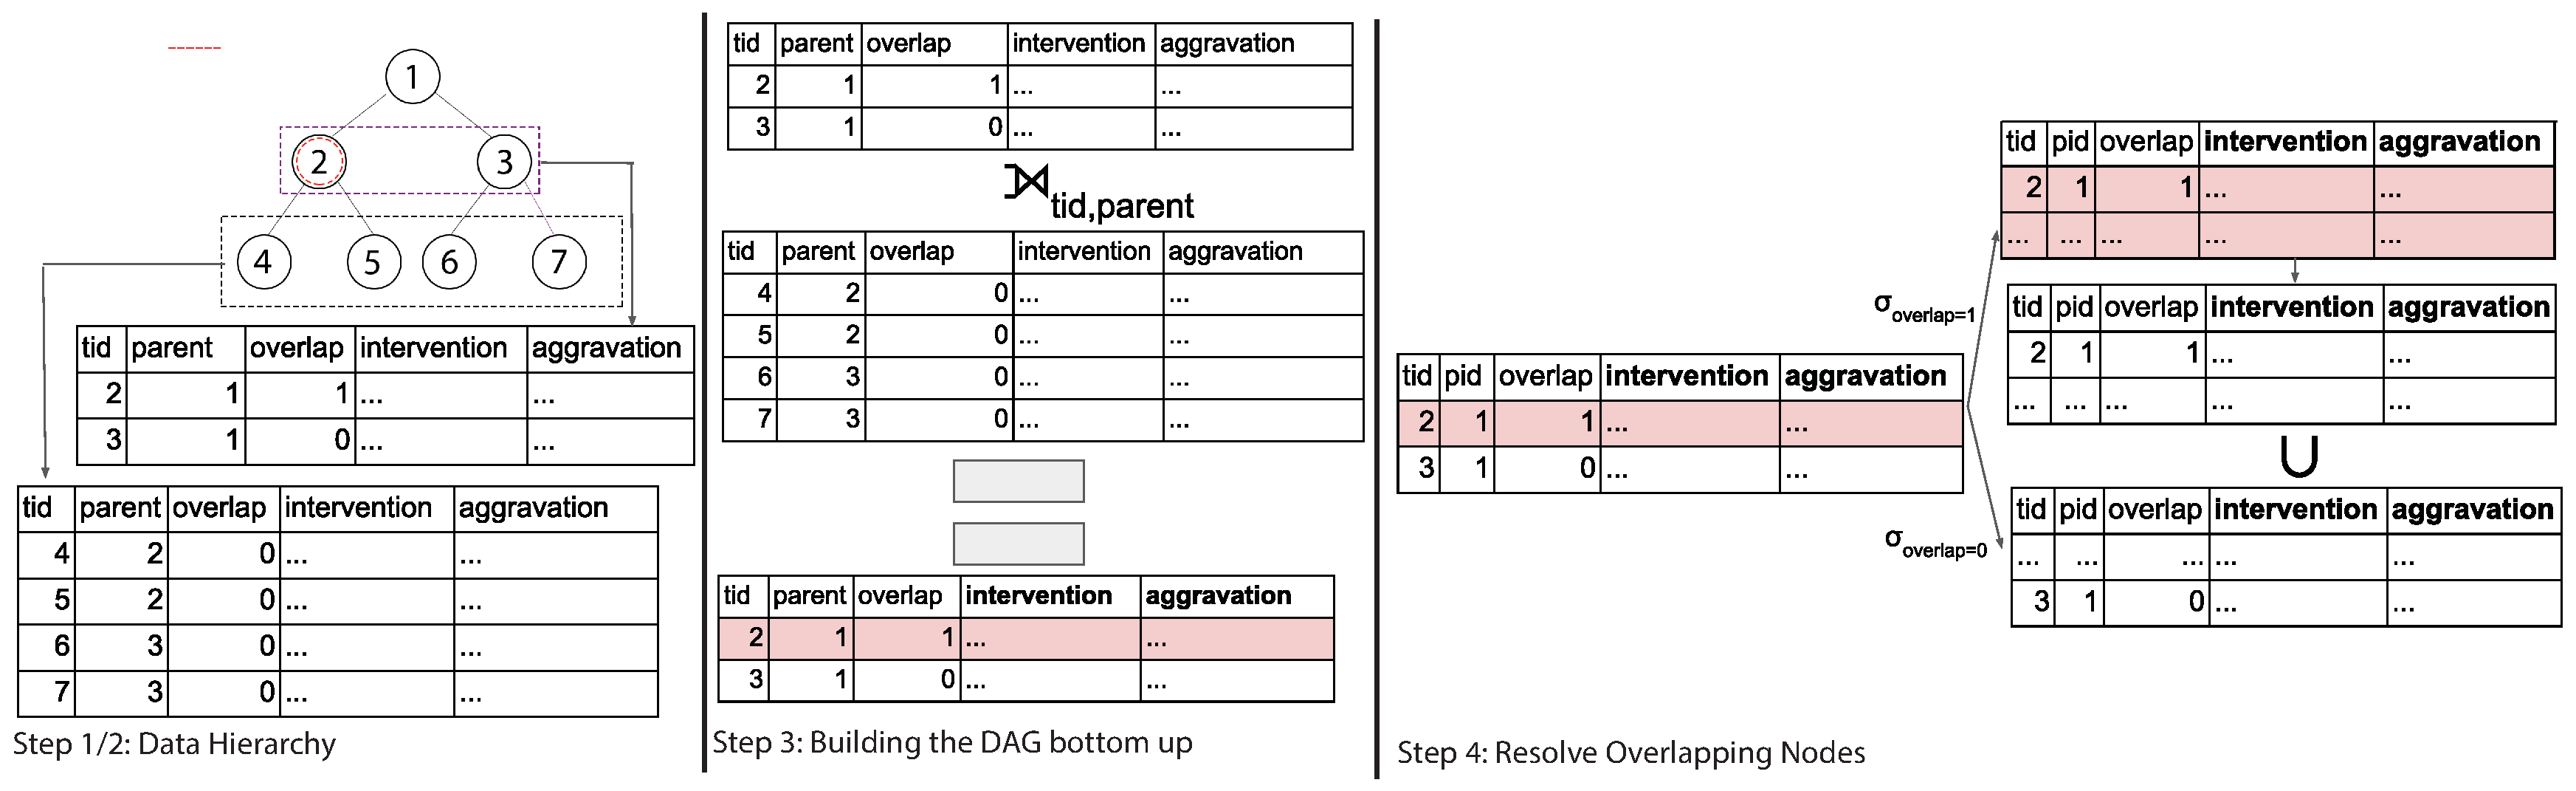
\includegraphics[width=\textwidth]{images/steps}}
\caption{Finding Spatial Explanation. The red dotted lines represent nodes which have children with overlapping tuples.}
  \label{fig:steps}
\end{figure*}


\subsubsection{Step1: Spatial Partitioning/Clustering}
There are several approaches to cluster data. Each clustering approach has a large impact on the resulting explanations. In order to understand the issues with explanations using spatial clustering, the hierarchical intervention approach can easily plug-in an existing clustering method and their impacts are studied in Section~\ref{sec:evaluation}.

%{\bf R-Tree} An R-Tree is a data structure which is commonly used for spatial data indexing. The idea behind the R-Tree is similar to the idea behind a binary tree i.e. It is faster to query data if it is stored in the form of a hierarchy\cite{guttman1984r}. In an R Tree, this hierarchy exists in the form of Minimum Bounding Rectangles(MBR). The top level of an R Tree consists of a set of MBRs which cover a large spatial area. Each MBR can now be subdivided into further MBRs which makes up the second level of the tree and so forth. At the leaf nodes of the tree, each node consists of a single object in our underlying data.


%{\bf R*-Tree} R* Tree is a variation of R-Tree\cite{beckmann1990r}. The objective of an R*-Tree is to minimize overlaps and coverage in an R-Tree. It also optimizes for margin and area. The idea behind R*-Tree which helps in achieving its objective is to use the perimeter of the MBR as a heuristic when splitting and creating R-Trees.

%{\bf K means} K means clustering is an algorithm designed to cluster a group of points \cite{macqueen1967some}. As the name suggests, the user decides the number of clusters that he/she wants. $K$ represents the number of clusters. The algorithm randomly selects $k$ seed points. The seed points can also be selected using a heuristic to improve the clustering. The points closest to each of the seed points form clusters. The k means algorithm is iterative. Which means it does not end there. The centroids of the clusters are used as new seed points and the process is repeated until the centroids are constant.


% TODO Add reference to greedy hierarchical clustering
% Let $D$ be our spatial dataset. Let $P$ be a set of distinct polygons over our dataset $D$. We define a set of distinct clusters of polygons $P_h$. The polygons can be clustered in many different ways but we used greedy hierarchical clustering because of its speed and relevance to the problem. Let $C$ be the set of centroids in $P$ i.e. $\forall p_i \in P$, $c_i$ is the centroid for $p_i$, where $c_i \in C$. We define a set of $n$ levels, $L = \{l_1, l_2,...,l_n\}$. We represent each centroid in $C$ on a cartesian plane where $x_i$ is the first dimension of the centroid $c_i$ and $y_i$ is the second dimension of the centroid $c_i$. Let $x_{min}$, $x_{max}$ be the minimum and maximum value for $x_i$ respectively. Let $y_{min}$, $y_{max}$ be the minimum and maximum values of $y_i$ respectively. There is a radius associated with each level in $L$. Let $r_i$ be the radius for level $l_i$ in $L$, We can define $r_i$ in general as,
% $$r_i = \frac{\sqrt{(y_{max}-y_{min})^2+(x_{max}-x_{min})^2}}{2^{i-1}}$$

% The set of clusters,$G_i$, for level $l_i$ can be defined as $G_i=\{p_k|(x_k^2 + y_k^2 < r_i^2)\}\forall p_k \in P$. Any possible set cover of $P$ in $G_i$ can now be considered for inclusion in $P_h$. One implementation of this approach is covered in Section~\ref{sec:hie_impl}


% \subsection{Hierarchical Greedy Clustering}
% Hierarchical Greedy Clustering is a popular algorithm in data visualizations because of its speed \cite{hgclustering}. The idea behind this algorithm is to randomly select points and create clusters around them.

% Let $D$ be our spatial dataset. Let $P$ be a set of distinct polygons over our dataset $D$. We define a set of distinct clusters of polygons $P_h$. Let $C$ be the set of centroids in $P$ i.e. $\forall p_i \in P$, $c_i$ is the centroid for $p_i$, where $c_i \in C$. We define a set of $n$ levels, $L = \{l_1, l_2,...,l_n\}$. We represent each centroid in $C$ on a Cartesian plane where $x_i$ is the first dimension of the centroid $c_i$ and $y_i$ is the second dimension of the centroid $c_i$. Let $x_{min}$, $x_{max}$ be the minimum and maximum value for $x_i$ respectively. Let $y_{min}$, $y_{max}$ be the minimum and maximum values of $y_i$ respectively. There is a radius associated with each level in $L$. Let $r_i$ be the radius for level $l_i$ in $L$, We can define $r_i$ in general as,
% $$r_i = \frac{\sqrt{(y_{max}-y_{min})^2+(x_{max}-x_{min})^2}}{2^{i-1}}$$

% The set of clusters,$G_i$, for level $l_i$ can be defined as $G_i=\{p_k|(x_k^2 + y_k^2 < r_i^2)\}\forall p_k \in P$. The algorithm for the implementation of this approach is covered in Section~\ref{sec:hie_impl}.

% Greedy Hierarchical Clustering turned out to have a drawback when we use it for explanations. It selects seed points randomly. This means that in each level, the clusters can be highly imbalanced. We compared this approach to K means(Voronoi partitioning)\cite{hartigan1979algorithm,aurenhammer2000voronoi}, R Tree\cite{guttman1984r} and R* Tree\cite{beckmann1990r}.

The main idea behind the hierarchical intervention approach, regardless of the partitioning algorithm, is to help us in increasing the domain for our degree of explanation. Since intervention is a subset of this approach, the domain is at least as large as that for intervention. After we have partitioned our data, each partition can be used as a predicate for aggravation and/or intervention.

\subsubsection{Step2: Hierarchical Dataframes Construction}
In our implementation of the system, we use the programming paradigm provided by Apache Spark. This involves using dataframes for processing. Dataframes resemble tables in a traditional RDMS. Each cluster in our spatial hierarchy is represented as a node in a tree. Each level of the tree is encapsulated as a dataframe. Each node has an ID associated with it. A tuple in our dataframe contains the ID of the node, the ID of the parent node, a column representing the overlap bit, columns representing the aggregates of the attributes, columns representing the aggravation/intervention for each query in our observation, and a column for the final values of aggravation/intervention after evaluating the arithmetic operation that represents our observation. 

The spatial hierarchy that we construct in step 1 of our algorithm is already a DAG since it takes the form of a tree. But for the next few steps, the DAG that we use is based on the dataframes. Instead of calculating aggravation and intervention for each tuple in our set of dataframes, we can use the values calculated in the leaf dataframe to build up the explanations.

\subsubsection{Step3: Building up the DAG}
Aggravation and Intervention are very expensive operations. In order to create a system for explanations which performs well, we need to reuse calculations. Thats the main reason we constructed our DAG in the first place. The intervention/aggravation values stored in one level of our DAG can be used one level above. We use the associative property of aggregate functions like sum and count to build our DAG bottom up. We use the group and join operations to implement this. The tuples at one level are grouped based on the parent id and left joined with the tuples at the parent level based on the node id and parent id of the child and parent dataframes respectively. 

Our system is designed to work with arbitrary clustering algorithms. Some of the clustering algorithms like K-Means have no overlapping tuples in the clusters with others like R-Tree have partitions with overlaps. In our spatial hierarchy if a node has child nodes with overlapping points, the overlap bit for that node is set to $true$. Using our build up approach so far, these nodes contain inaccurate values of intervention and aggravation. Before building the DAG further up these values need to be fixed.

\subsubsection{Step4: Overlap Resolution}
Depending of the type of spatial partitioning, some nodes in our DAG have incorrect values of aggravation/intervention stored in the dataframe. These are nodes where the overlap bit is $true$. Since we are using dataframes, we cannot update individual tuples. Instead, we create two dataframes out of the original. One containing tuples where the overlap bit is true and one containing the rest of the tuples. The aggravation/intervention and aggregates for the first dataframe are recalculated. Finally both the dataframes are combined using union and the old dataframe is replaced with the new one in the DAG. Using this sequence of operations, we can reduce the number of calculations. Since our dataframe now contains accurate information, we can resume building the DAG further up.


\subsubsection{Step5: Ranking Explanations}
\label{sec:extending_hi}

%In order to get the most out of Hierarchical Intervention, we introduce two new metrics: Intensity and Influence.
%
%\textbf{Intensity:}
%\label{sec:intensity}
%%What is relevance
%We define intensity as a metric which measures the standalone value of the explanation. The relevance metric borrows a lot from our definition of aggravation. It might be convenient to think of a web search engine when we are looking at the intensity metric. When we use a search engine, we provide a search term as a query. The search engine looks at all the pages in its database and returns the results in order of relevance. The top results in the search engine may not have a significant effect on the entire web if they were to be removed. However, the top result in the search engine has the highest relation to the data. For example, the top result for a search engine which uses tf-idf might be a page containing the highest frequency of the search term\cite{robertson2004understanding}.
%
%%Formal definition of relevance
%Let $D$ be our dataset. Let $\phi$ be our candidate explanation. Let $R$ be the function which maps our dataset to the value of our observation. Then we can define intensity as,
%$$intensity = |R(\sigma (D)) - R(\sigma_\phi (D))|$$
%
%\textbf{Influence:}
%\label{sec:influence}
%% What is influence
%We define influence as a metric which measures the value of the explanation compared to the entire dataset. The influence metric borrows from our definition of intervention. The influence metric measures how much the observation would be affected if we remove the data related to our explanation(the \textit{influence} of our explanation on the observation). We can use the analogy of the search engine again here. One of the earliest algorithms used by Google to rank webpages used links to other pages\cite{brin1998anatomy}. The page which was linked the most on a variety of websites was ranked higher. If you remove a highly relevant page, many other pages might not exist. Influence uses the same principle.
%
%%Formal definition of influence
%Let $D$ be our dataset. Let $\phi$ be our candidate explanation. Let $R$ be the function which maps our dataset to the value of our observation. Then we can define relevance as,
%$$influence = |R(\sigma(D)) - R(\sigma_{\neg \phi} (D)) |$$
%
%The greater the value of influence, the more its impact on the observation.
%
%Our evaluation metrics suggest that influence and intensity explain data in different ways. Explanations with higher influence tend to give predicates which cover a larger area while explanations with higher intensity tend to give predicates which cover a small area. We can balance out these two metrics according to the preferences of the observer. We define the \textit{explanation index}, $\epsilon$ as:
%$$\epsilon = \alpha \times influence + (1-\alpha) \times intensity$$
%$\alpha$ is the \textit{explanation coefficient}. It is a variable whose value is decided by the user.
%
%Explanations given by Hierarchical Intervention can be ranked on the basis of the explanation index.

%\pagebreak
%\section{The automated framework}
%Fig.~\ref{fig:framework} shows the system diagram for our solution which uses hierarchical intervention. We take inputs in the form for aggregate queries. An arithmetic expression encapsulates the relationships between these queries. On the other hand, we have a spatial dataset. We use clustering/partitioning to create a hierarchy out of our spatial data. Depending on the hierarchy that we have created and our inputs, we perform aggravation and intervention. The results of aggravation and intervention are used to in a ranking system based on an explanation index. The explanation index measures the candidate explanations as a linear relationship between aggravation and intervention. How much each explanation approach is weighted in the explanation index is under the control of the data analyst. Finally, the top results are used for visualization. We have created a web-based GUI to display these kinds of explanations.
\subsection{User interface}

\subsection{Explanation engine}

\section{EXPERIMENTS}
\label{sec:evaluation}
%Why we need evaluation\label{sec:relevance}
The main contribution of this paper is to introduce a new approach for explanations(Hierarchical Intervention). We evaluate this new approach in a number of different ways. We perform qualitative evaluation and speed/scalability evaluation.

\begin{figure}[H]
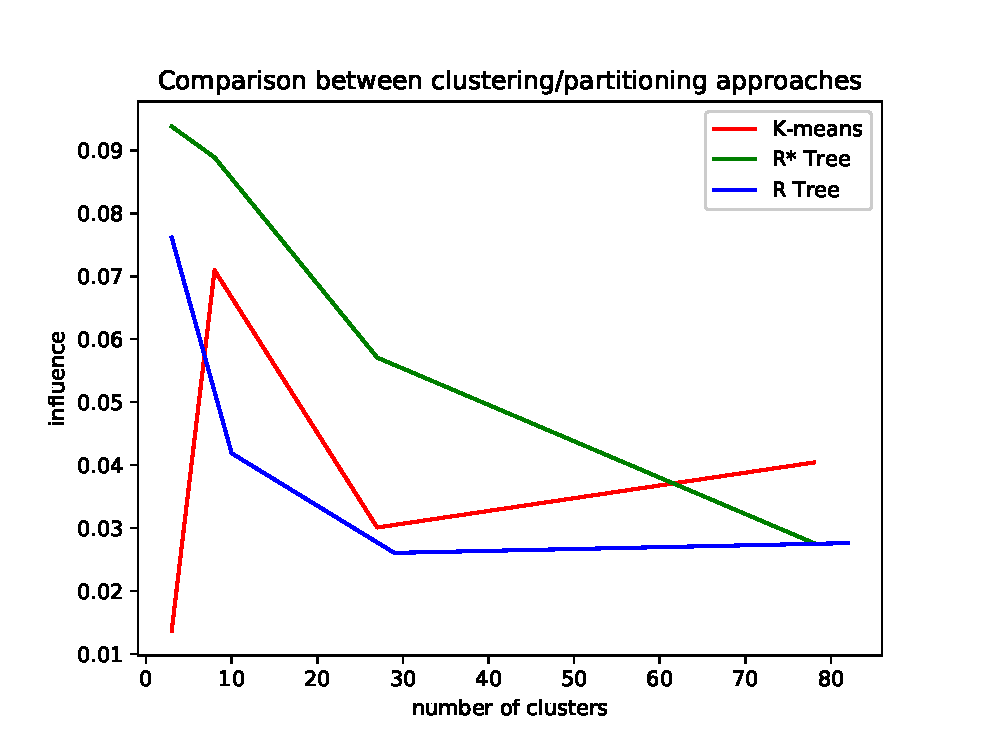
\includegraphics[width=\columnwidth]{images/clustering_comparison}
\caption{Comparison of Influence against number of clusters for K-Means, R-Tree and R*-Tree}
\label{fig:clustering_comparison}
\end{figure}

In order to compare the different clustering techniques that we use in hierarchical intervention, we did a couple of experiments. Our solution relies on the fact that the higher the influence or intensity are a measure of the value of our explanations. We used a number of observations on the NYC TLC data to see how each clustering technique fares against the others.

\textbf{Experimental Setup}. 
In our evaluation, we will use both single-machine and multiple-machines environments. 
In the single-machine environment, we use one machine with an i7 6400 3.5 GHz CPU and 8GB of RAM. 
In a multiple-machines environment, we take Google Compute Engine as our cluster. 
The cluster has 4 nodes and each machine has 1 vCPU and 3.5GB RAM.

{\bf Dataset}. 
In our experiment, we use the yellow and green taxi trip records as our dataset. 
This dataset includes the pick-up and drop-off location of the taxi trips and the properties for each trip, such as fare, payment method, etc,. The dataset is organized in a monthly way that each file in the dataset stores the trips within one month.
%The dataset used for this experiment was the NYC TLC data for January 2016. This data contains ~10 million trips.

%\textbf{Experimental Setup}. We performed the evaluation on the first 5 months of data from the NYC yellow cab dataset from 2016. The data spanned ~ 50 million trips. The $k$ for our evaluation was $5$. This value was chosen after a series of experiments. We wanted the size of each partition to be large enough to support our generalization assumption. If the solution space for evaluation is small, it leads to inconsistent results. Each month represented a partition for k-folds evaluation. According to our analysis, we found that the approach works very well with low values of alpha. Fig.~\ref{fig:kfolds} shows some of the results of our evaluation for a number of observations. The lower the value of the relative distance, the better the results.

%\textbf{Experimental Setup}. The speed of each approach is simply the time taken to calculate the explanations. Since all the approaches are implemented on top of distributed systems, the time varies depending on the number of nodes used. We experimented with calculating explanations for 1,3, and 5 months in a distributed environment. For the cluster, we used Google Compute Engine nodes(1 vCPU, 3.5GB RAM, 4 nodes). All the nodes in our cluster had the same specifications. The Aggravation, Intervention and Hierarchical Intervention were tested on Apache Spark running on YARN while the Salient Features were generated with the Data Polygamy Framework running on YARN.

\subsection{Spatial partitioning methods}
\begin{figure}[h]
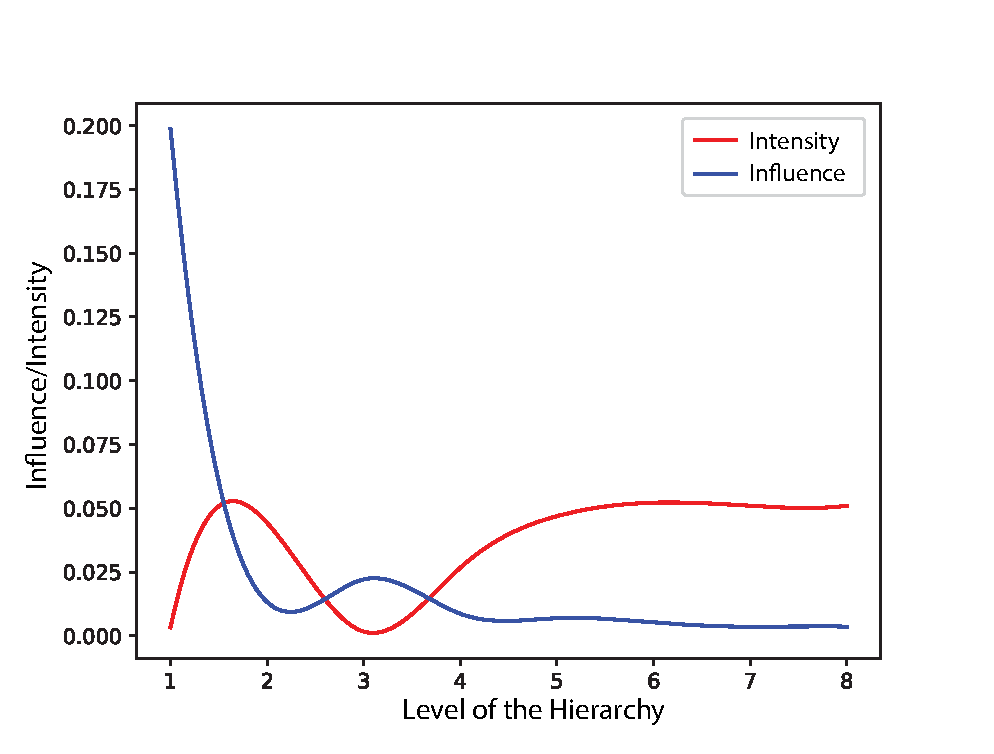
\includegraphics[width=\columnwidth]{images/hieint_passenger_count}
\caption{Comparison of Influence and Intensity against level of hierarchy with average passenger count as observation}
\label{fig:hieint_passenger_count}
\end{figure}
Spatial explanation requires to create spatial predicate which partition the whole dataset into different spatial partitions. In our evaluation, we consider three spatial partitioning methods, R-Tree, R* Tree and K-means. 
Fig. \ref{fig:clustering_comparison} shows the influence of different partitioning methods with different number of clusters. 
It shows that R-Tree and R* Tree partitioning are usually more stable than K- Means. The stability of the clustering technique is referring to its monotonicity of the explanation as a function of the number of clusters. Fig.~\ref{fig:hieint_passenger_count} shows the influence against the number of hierarchy levels where the observation is the average passenger count. The influence and intensity are closer to a sinusoidal curve than a exponential or logarithmic curve. Fig.~\ref{fig:clustering_comparison} shows another observation and a plot of the influence of R-Tree and R*-Tree as well. The influence as a function of the number of clusters is a lot more monotonic here. Furthermore, R* Tree has a higher influence on average compared to other approaches making it a lot more suitable for explanations.
%Reasons for selecting evaluation criteria
The qualitative evaluation that we define is based on K-Folds cross validation. The reason for selecting these evaluations is to measure how the top explanations provided by each approach fair as stand alone parts of data as well as their effects on the entire dataset as a whole. Other than qualitative analysis we look at the speed and scalability of each approach for performance evaluation.



%How does each approach compare
\textbf{Influence Comparison.}
Fig.~\ref{fig:influence_comparison} shows the comparison between the influence of different approaches. Salient features and Aggravation have a very low influence compared to Intervention and hierarchical intervention. This is because the explanations provided by those approaches cover a very small portion of the entire dataset. This makes removing the associated data have a negligible impact on the entire data.
\begin{figure}[h]
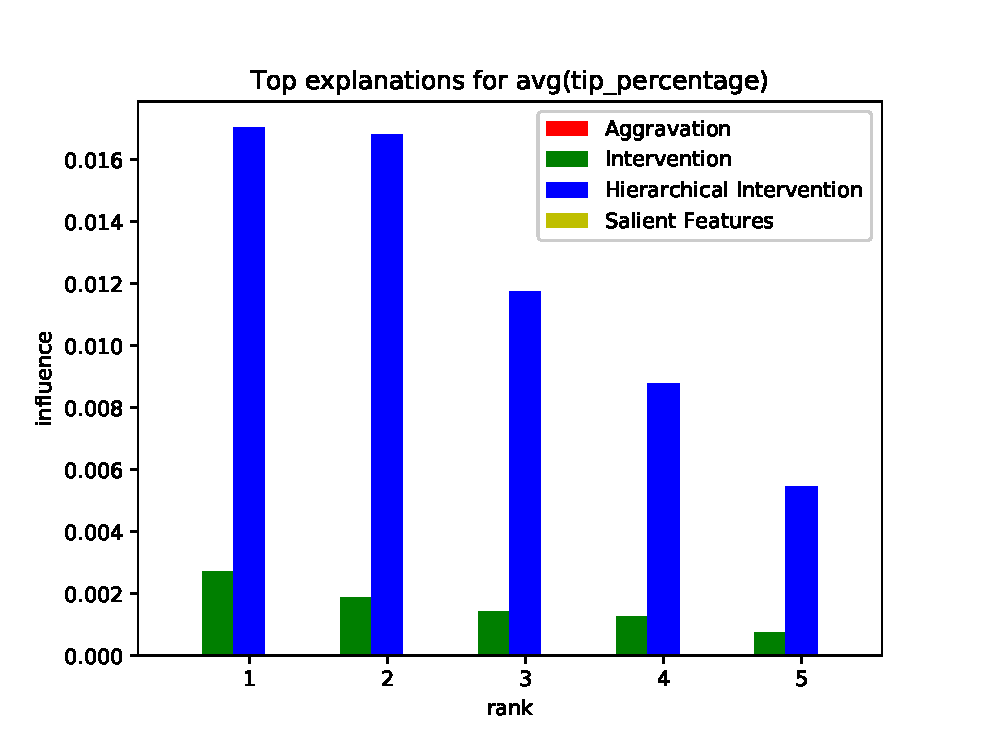
\includegraphics[width=\columnwidth]{images/Top_explanations_for_avg_tip_percentage_influence}
\caption{Influence for Spatial explanation for average tip percentage(Lower is better)}
\label{fig:influence_comparison}
\end{figure}

\subsection{K-Folds cross validation}
In order to qualitatively assess the solutions, we use K-Folds cross validation\cite{refaeilzadeh2009cross}. 
%\section{K-Folds Cross Validation}
K Folds cross validation is a technique for data evaluation\cite{kohavi1995study,refaeilzadeh2009cross}. The data is divided into $k$ parts. One of the parts is used as a training set and the remaining parts are used as test sets. The purpose of the training set is to model the data. Once we have a model, we can use it to classify and/or predict unseen data. The test set is used to evaluate how well the model was trained.

Since we do not have ground truth for our explanations, we have to make a compromise in terms of estimating how good our solution is. Our assumption here is that in general, a good explanation would stand out on unseen data i.e. given a good explanation on part of the data, it would give similar results on unseen parts of the data. This is the same assumption that was made by \cite{chirigati2016data} in their evaluation of the Data Polygamy framework. We split the data into $k$ parts. The data was divides by the month of the year. This is because there are specific observable patterns in each month, e.g. weekends have less density of trips than the weekdays for the dataset we evaluated. One of the parts is used to find the explanation(the training data). The rest of the data is the test data. We also calculate an explanation of the test data. The relative distance between the explanation index of the test data and the explanation index of the explanation provided by the training data when applied to the test data is used as a measure of evaluation.



\textbf{Experimental Setup}. We performed the evaluation on the first 5 months of data from the NYC yellow cab dataset from 2016. The data spanned ~ 50 million trips. The $k$ for our evaluation was $5$. This value was chosen after a series of experiments. We wanted the size of each partition to be large enough to support our generalization assumption. If the solution space for evaluation is small, it leads to inconsistent results. Each month represented a partition for k-folds evaluation. According to our analysis, we found that the approach works very well with low values of alpha. Fig.~\ref{fig:kfolds} shows some of the results of our evaluation for a number of observations. The lower the value of the relative distance, the better the results.

The relative distance in the K Folds cross validation represents how much the explanation impact changes when we look at the explanations in the context of unseen data. A relative distance of zero represents that the explanation has the same impact on unseen data as if we had seen the data. A relative distance of one would represent that the top explanation for the unseen data has nothing in common with the explanation of seen data. Let $e_{test}$ be the explanation index for the test set. Let $e_{train}$ be the explanation index for the training set. Then,

$$relative\_distance = \frac{|e_{test}-e_{train}|}{|e_{test}+e_{train}|}$$

The relative distance metric was chosen because of its nature of showing a steep decline when two solutions do not match. It is also ideal because it caters to the different types of observations that a user can specify. Since the observations in our system are defined as an arithmetic operation over aggregate queries, they do not have bounds on their values. Thus, it makes relative distance a useful metric for measuring similarity.

Here are the observations that we show in Fig.~\ref{fig:kfolds}:
\renewcommand{\lstlistingname}{Query}% Listing -> Algorithm
\begin{lstlisting}[language=SQL, caption=o1 for Fig.~\ref{fig:kfolds}, label=qry:o1]
Select count(*) as q1 
from data where payment_type=1;

Select count(*) as q2 
from data where payment_type=2;
Observation = q1/q2
\end{lstlisting}

\begin{lstlisting}[language=SQL, caption=o2 for Fig.~\ref{fig:kfolds}, label=qry:o2]
Select AVG(trip_distance) as q1 
where passenger_count=4;
Observation = q1
\end{lstlisting}

\begin{lstlisting}[language=SQL, caption=o3 for Fig.~\ref{fig:kfolds}, label=qry:o3]
Select count(*) as q1 
from data where vendorid=1;

Select count(*) as q2 
from data where vendorid=2;

Observation = q1/q2
\end{lstlisting}

\subsection{Precision and Recall}
% \begin{wrapfigure}{L}{0.5\textwidth}
%   \begin{center}
%     \includegraphics[width=0.48\textwidth]{outbreakheatmap.png}
%   \end{center}
%   \caption{A heatmap showing sythesized data}
%   \label{fig:synthesized_data}
% \end{wrapfigure}
% \begin{figure}[h]
% \includegraphics[width=\columnwidth]{outbreakheatmap.png}
% \caption{A heatmap showing sythesized data}
% \label{fig:synthesized_data}
% \end{figure}

Since it is very difficult to find datasets with the ground truth we used synthetic datasets to evaluate our solution\cite{maciejewski2009generating}. The synthetic dataset is fabricated using real data from Indiana Public Health Emergency Surveillance System. This data contains information about Patients in Indiana and their health issues over time and location. We can calculate precision and recall using this data\cite{powers2011evaluation}. The data is synthesized in such a way that it shows similar patterns to the actual data. Synthetic data related to outbreaks of certain diseases is synthesized into this data. In order to evaluate our system, we used the temporal component of the outbreak and the type of disease as our observation. To be specific, the synthetic data consisted of an outbreak of Gastrointestinal infection in July. Our observation was the ratio of the number of gastrointestinal infection incidents between June and July when there's an infection against the number of gastrointestinal infection incidents between June and July in synthesized data where there wasn't an outbreak. Precision and Recall was calculated by comparing the areas of the top ten explanations related to the ground truth with the approximate area covered by the outbreak data. We cannot use the individual points to calculate precision and recall because there is a lot of data unrelated to the outbreak which occurs in proximity. To put things into context, each instance of the synthesized data contains ~2 million records. The data related to the outbreak consists of a few dozen records. Fig.~\ref{fig:synthesized_data} shows a heatmap of all the points in the synthesized data. The outbreak for this particular instance only affects a small part of Indiana to the North West just below Lake Michigan. Fig.~\ref{fig:precisionrecall} shows the points representing the outbreak as well as some of the top polygons returned using Hierarchical Intervention. While our system is designed to work fast on partitioning techniques with no overlaps like K-Means and Greedy Hierarchical Clustering. Some of the clustering approaches that we use which give better results do have overlaps. Thus we used R*-Tree partitioning in our example. The candidate explanations provided by this partitioning techniques can have spatial overlaps.

% \begin{figure}[h]
% \includegraphics[width=\columnwidth]{precisionrecall.png}
% \caption{Synthetic Outbreak data. The circles show the ground truth while the polygons show the relevant explanations produced by our system}
% \label{fig:precisionrecall}
% \end{figure}

Precision can be evaluated by the following equation:
$$Precision = \frac{E \cap O}{E}$$
where $E$ is the area represented by our polygons and $O$ is the area represented by the Outbreak points.

% don't understand the definition (why it is defined as this?)
For calculating recall, we can use the actual outbreak points since it doesn't require false positives.
$$Recall = \frac{true\_positives}{false\_negatives}$$

\begin{table}[]
    \centering
    \caption{Precision and Recall}
    \begin{tabular}{|c|c|c|c|}
        \hline
        Precision & 0.31 & 0.01 & 0.0003\\ \hline
        Recall &  0.74 & 0.04 & 1\\ \hline
    \end{tabular}
    \label{tab:precision_and_recall}
\end{table}


\subsection{Comparison}
We compared the precision and recall of Hierarchical Intervention with Aggravation and Intervention.
\\
\textbf{Aggravation}. We used the same observation for aggravation that we did for Hierarchical Intervention. From the top ten explanations, only one of the explanation was able to predict one of the 27 correct tuples in the ground truth.
$$Precision = 0.01$$
$$Recall = 0.04$$


\textbf{Intervention}. Finally, Intervention was used to find an explanation. Since there was only one hospital in the area of the outbreak, Intervention was able to provide that hospital as a relevant predicate in an explanation. This resulted in all the ground truth points being included in the explanation! However, since there are a large number of tuples related to this predicate, it resulted in a low precision.

$$Precision = 0.0003,\ Recall = 1$$


% \begin{wrapfigure}{r}{0.5\textwidth}
%   \begin{center}
%     \includegraphics[width=0.48\textwidth]{precisionrecall.png}
%   \end{center}
%   \caption{Synthetic Outbreak data. The circles show the ground truth while the polygons show the relevant explanations produced by our system}
% \label{fig:spatial_spatial_vertical}
% \end{wrapfigure}



% \textbf{Influence and Intensity for Hierarchical Intervention}
% \begin{figure}[H]
% 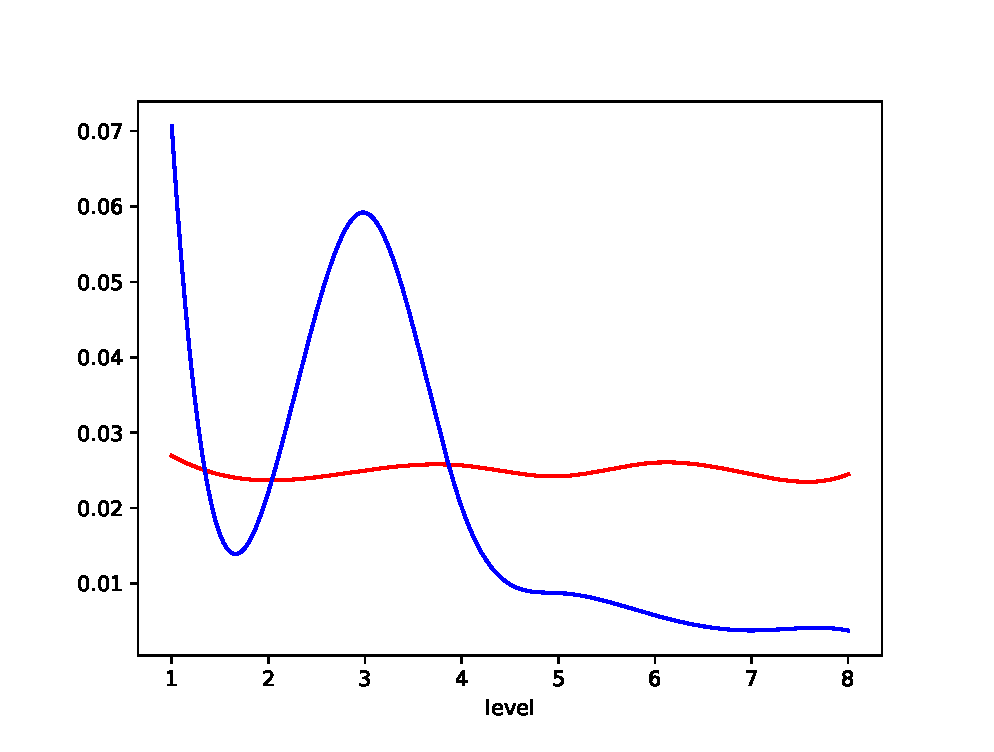
\includegraphics[width=\columnwidth]{heiint_tip_percentage}
% \caption{Comparison of Influence and Intensity against level of hierarchy with average tip percentage as observation}
% \label{fig:hieint_tip_percentage}
% \end{figure}




% \begin{figure}[H]
% 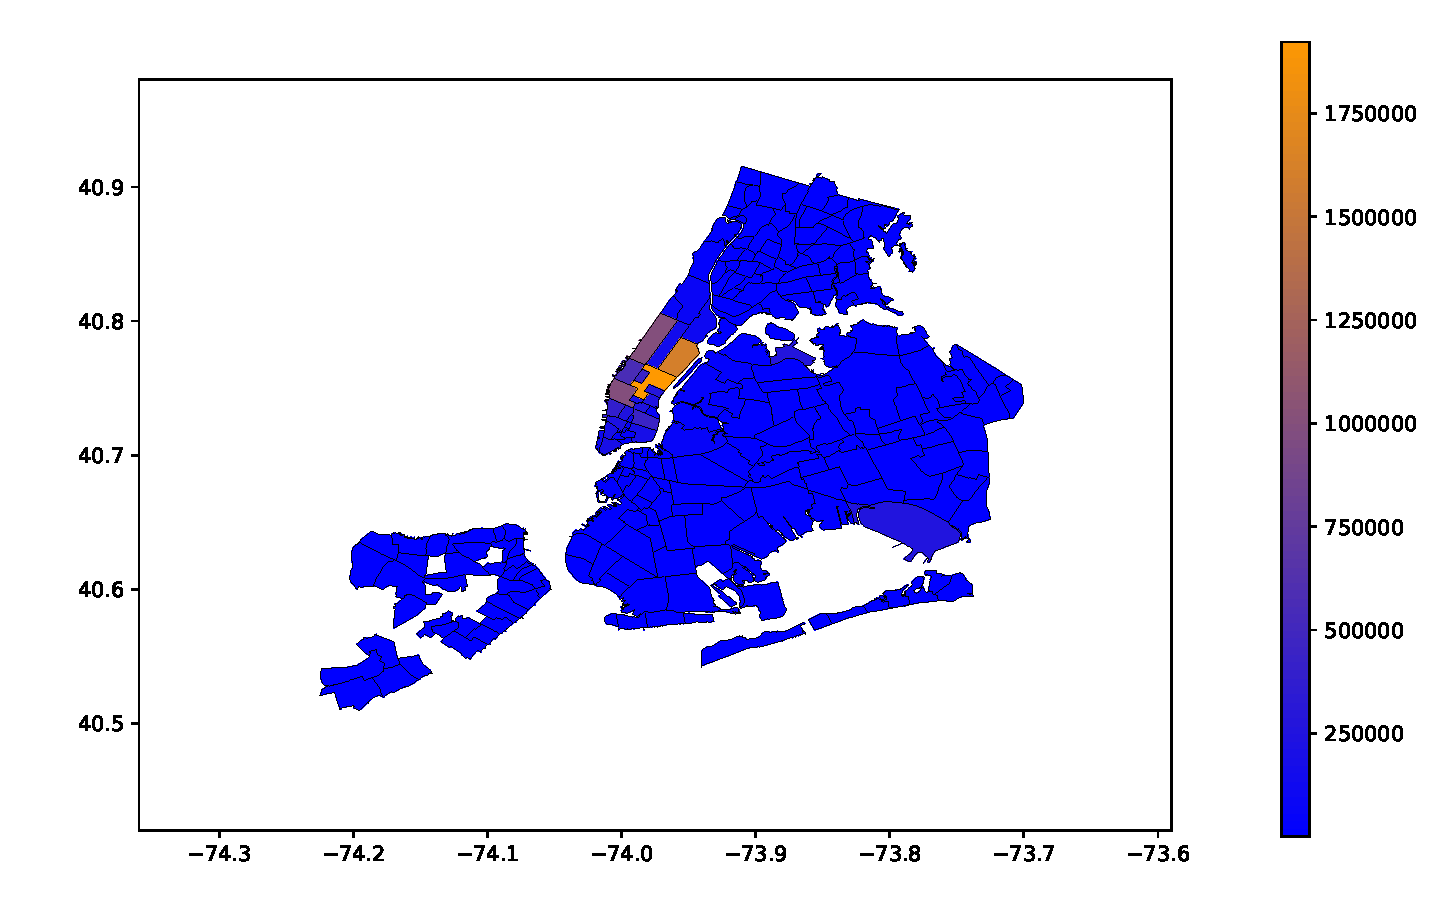
\includegraphics[width=\columnwidth]{count_initial}
% \caption{The number of trips for each zone by pickup zone}
% \label{fig:count_initial}
% \end{figure}

% \begin{figure}[H]
% 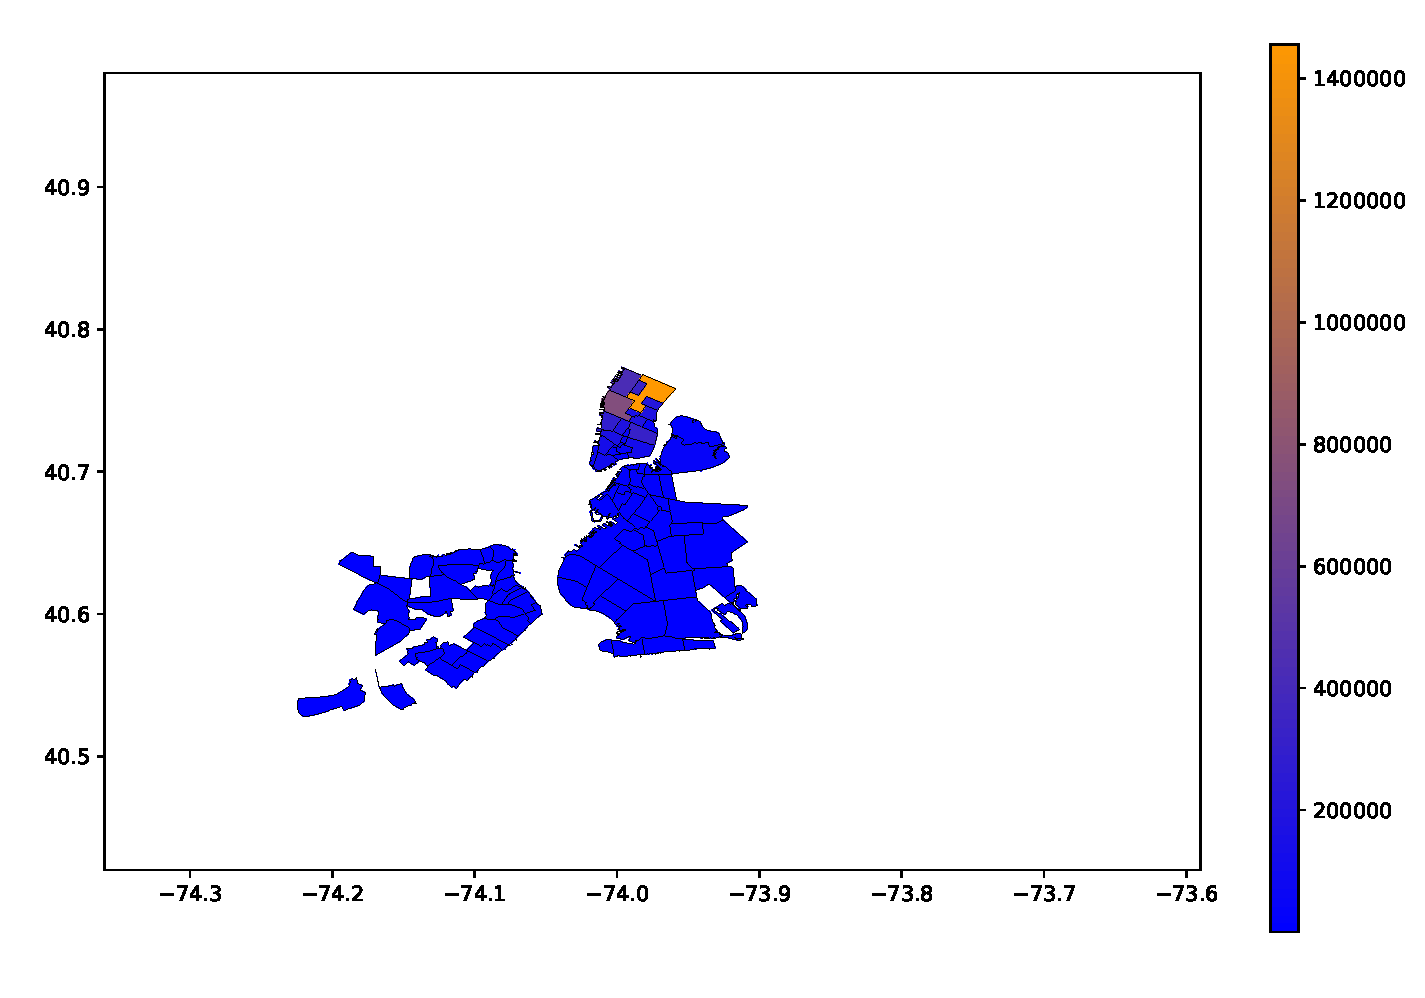
\includegraphics[width=\columnwidth]{top_level_2}
% \caption{Number of rows that represent the top explanation for average tip percentage at level 2}
% \label{fig:top_level_2}
% \end{figure}

% \begin{figure}[H]
% 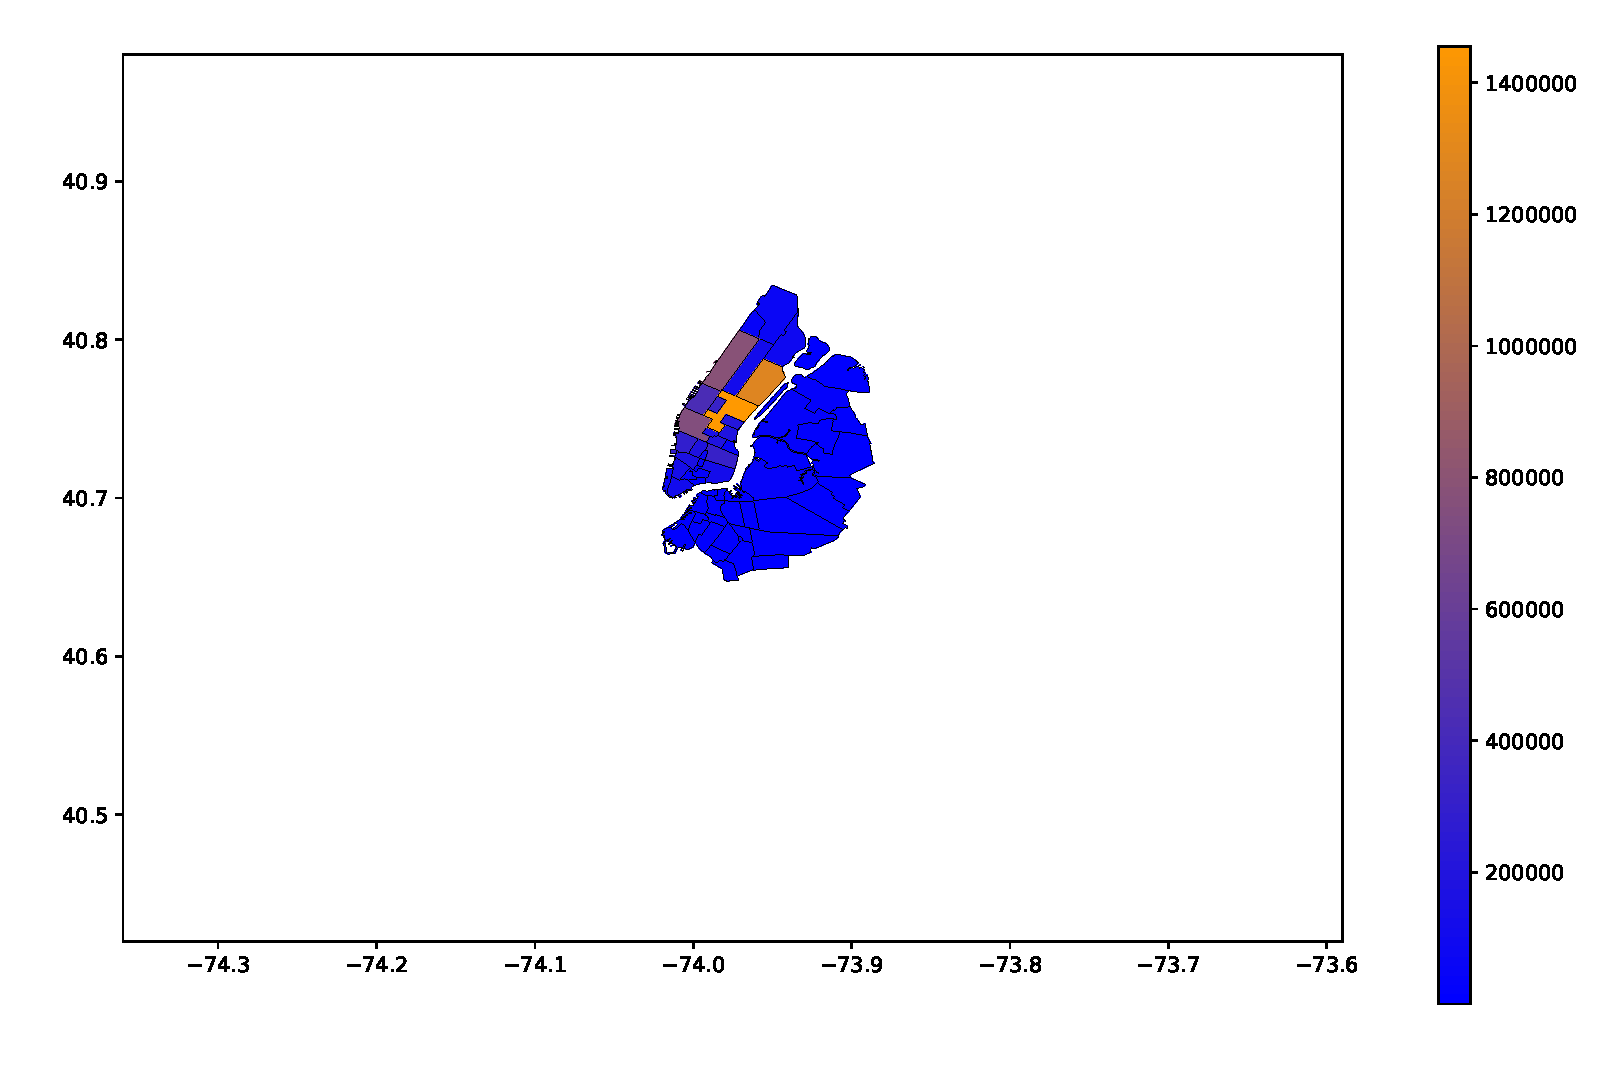
\includegraphics[width=\columnwidth]{top_level_3}
% \caption{Number of rows that represent the top explanation for average tip percentage at level 3}
% \label{fig:top_level_3}
% \end{figure}

% \begin{figure}[H]
% 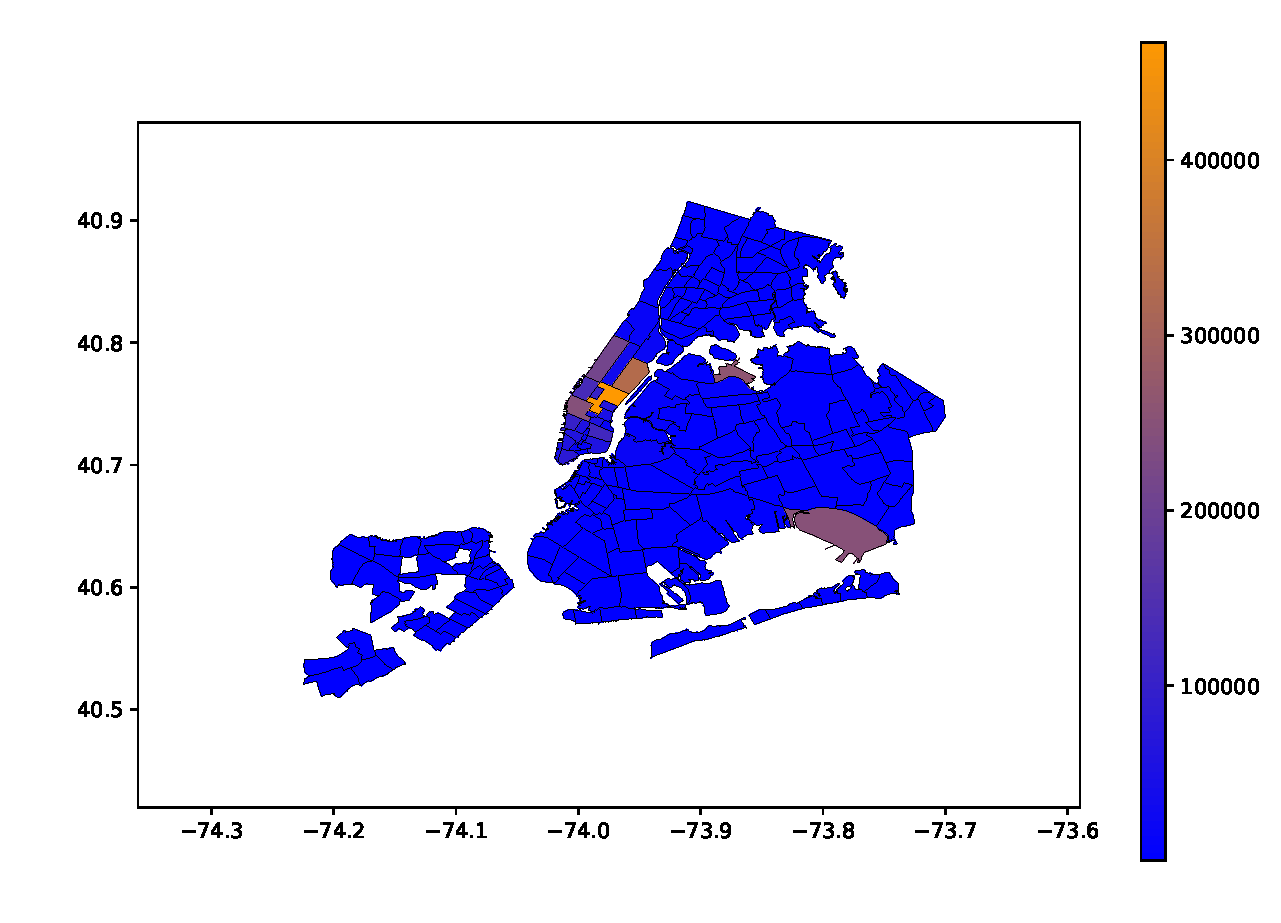
\includegraphics[width=\columnwidth]{level_3_removed}
% \caption{The cartogram for the data when we remove he level 3 explanation}
% \label{fig:level_3_removed}
% \end{figure}


\subsection{Speed and Scalability}
\label{sec:speed}
The speed of each approach is simply the time taken to calculate the explanations. The time varies depending on the size of the data. For performance evaluation, we used the NYC TLC data for 2016. The data is divided into months. As we increase the number of months to be processed, the time taken for each approach increases almost linearly for aggravation, intervention and hierarchical intervention. For salient features, the time increases slightly exponentially. The results of our evaluation are displayed in Fig.~\ref{fig:performance}

\textbf{Experimental Setup}. The speed of each approach is simply the time taken to calculate the explanations. Since all the approaches are implemented on top of distributed systems, the time varies depending on the number of nodes used. We experimented with calculating explanations for 1,3, and 5 months in a distributed environment. For the cluster, we used Google Compute Engine nodes(1 vCPU, 3.5GB RAM, 4 nodes). All the nodes in our cluster had the same specifications. The Aggravation, Intervention and Hierarchical Intervention were tested on Apache Spark running on YARN while the Salient Features were generated with the Data Polygamy Framework running on YARN.
\begin{figure}[h]
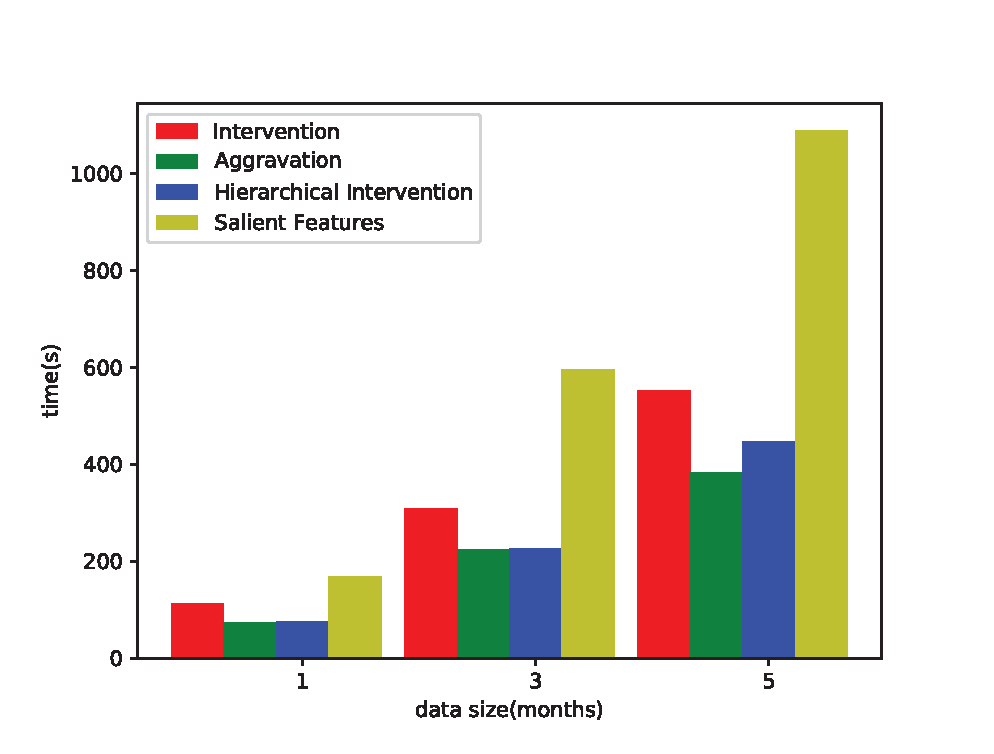
\includegraphics[width=\columnwidth]{images/performance}
\caption{Time taken by each approach as we increase the size of data}
\label{fig:performance}
\end{figure}
The run times that were observed can be explained as follows. Aggravation takes the least amount of time of the compared approaches. Intervention costs more than aggravation because it includes the additional step of calculating statistics for the attributes as well as iterating the table. Hierarchical Intervention takes more time than aggravation but less time than intervention. This is because of several factors. One of the factors is that when we are using intervention and aggravation, we are using several attributes, on the other hand, hierarchical intervention only uses the spatial attribute. On the other hand, we are creating a hierarchy. The in the case of this analysis we only used one query as the observation for the sake of comparison. However, multiple queries can affect the comparison as well. The time taken by Salient Features is also affected by a number of factors. First, the implementation of the salient features that we use is the one used in the Data Polygamy Framework \cite{chirigati2016data}. This approach uses the MapReduce framework. The other approaches use the Spark framework. Since Spark makes use of an execution plan which is more efficient than MapReduce, it is a factor in the slower runtime of the Salient Features approach. Thus, when comparing salient features to the other approaches, this can be considered something similar to black box testing. The most expensive computation step in salient features is the interpolation step which doesn't occur in the other approaches.


% \begin{figure}[H]
% 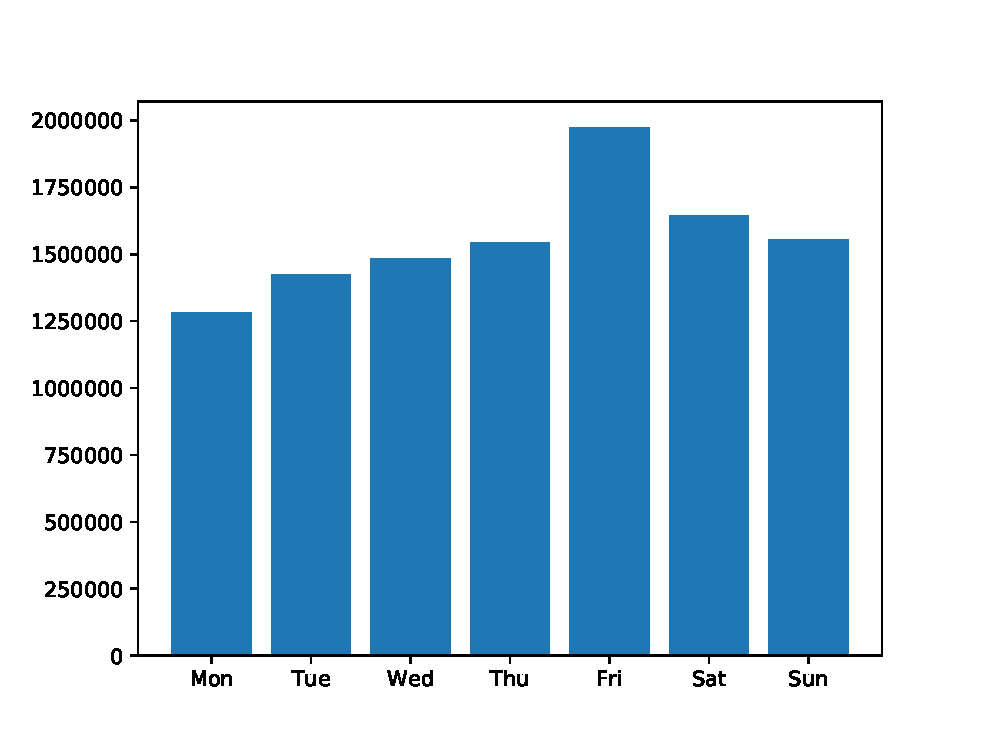
\includegraphics[width=\columnwidth]{day_comparison}
% \caption{Number of trips against trip day}
% \label{fig:day_comparison}
% \end{figure}

\section{CONCLUSION AND FUTURE WORK}
\label{chp:concl}
In this paper, we looked at different approaches for spatial explanations for arbitrary observations. We built an approach called Hierarchical Intervention. According to our evaluation, our approach outperforms aggravation and intervention in precision while it outperforms aggravation in recall. If we look at our approach from the context of a data analyst, it is designed to provide an advantage over traditional data analytics using relational database systems. The reason for this is because we use programming paradigms for distributed processing. Even though our implementation is designed to work on Apache Spark, the paradigms used may be useful for future distributed processing systems like GOLEM which have an even larger processing scope \cite{golem2018}. In addition to saving valuable time for data analyst, our system is also useful for reducing the scope of work for the analyst. The proposed system can be used as a search engine much like Google where the analyst uses observations instead of search terms and the system comes up with explanations instead of web pages. Instead of looking at the entire data, the analyst can look at a small subset represented by these explanations to find what they are looking for.

There are a number of improvements that can be made on top of our proposed approach that we weren't able to implement due to the lack of time or availability of datasets with the ground truth. One interesting idea is to use influence and intensity as parameters of perceptrons in a neural network\cite{grossberg1988nonlinear,widrow199030}. The neural network can be trained to explain specific datasets by using ground truth.
Many spatial datasets that we find also have a temporal component. Our system does not handle the temporal aspect of the data. An improvement that can be made to our approach is to use time range as a secondary component of our candidate explanations. We can build a temporal hierarchy in the same way we build a spatial hierarchy. The spatiotemporal hierarchy can be represented as a pyramid instead of a tree.
If we extend our idea of the spatiotemporal system to a neural network, we can think of it from the perspective of a recurrent neural network\cite{chung2016hierarchical}. It might also help to use Long Short Term Memory(LSTM) model to encapsulate the value of explanations at levels of the hierarchy which are far apart \cite{hochreiter1997long}.
Since influence and intensity are expensive operations, the time complexity of the network should also be taken into account and heuristics should be used where necessary when using approaches with a lot of inputs.



\newpage

\bibliographystyle{acm}
\bibliography{dis} 

\end{document}
